%% LyX 2.1.4 created this file.  For more info, see http://www.lyx.org/.
%% Do not edit unless you really know what you are doing.
%\documentclass[12pt,a4paper,english,3p]{elsarticle}
\documentclass[12pt,a4paper,english]{article}

%\usepackage[english]{babel}%muda chapter para capítulo
\usepackage[utf8]{inputenc}%escrever os acentos diretamente, sem macro
%\usepackage[T1]{fontenc}%muda a codificação da fonte, podendo copiar textos
\usepackage{hyperref, graphicx}
\hypersetup{colorlinks=true,linkcolor=blue}%, linktocpage}
\usepackage{indentfirst}%paragrafo

\usepackage{ae,aecompl}
\usepackage[T1]{fontenc}
%\usepackage[latin9]{inputenc}
%\usepackage[utf8]{inputenc}
\pagestyle{plain}
\setlength{\parskip}{\smallskipamount}
\setlength{\parindent}{0pt}
\usepackage{amsmath}
\usepackage{amssymb}
\usepackage{babel}
\usepackage{xcolor}
\usepackage{amsmath, amssymb, float, subfig, mathabx}
\usepackage{booktabs}  % For professional table rules (\toprule, \midrule, \bottomrule)
\usepackage{siunitx}
\usepackage{subcaption}
%\makeatletter
%\usepackage[notcite,notref]{showkeys}
%\usepackage{biblatex} 
%\addbibresource{bibliography.bib}
\usepackage{authblk} % Standard package for multiple affiliations

\usepackage[
    letterpaper,                % Paper size (use 'a4paper' if in Europe/Asia)
    top=1in,                    % Top margin
    bottom=1in,                 % Bottom margin
    left=1in,                   % Left margin
    right=1in,                  % Right margin
    heightrounded,              % Rounds textheight to a whole number of lines (prevents underfull vbox errors)
    bindingoffset=0in           % Set to 0.25in only if you plan to bind it like a book
]{geometry}


\title{Revisiting drops impacting a sieve}

% Assign footnote markers [1], [2], etc.
\author[a]{D. A. Aguiar}
\author[c]{A. S. Pereira}
\author[b]{R. L. Thompson}
\author[a]{C. M. Oishi}
\author[a]{I. L. Palhares Junior}


% Define the affiliations
\affil[a]{Departamento de Matemática e Computação, Faculdade de Ciências e Tecnologia, Universidade Estadual Paulista 'Júlio de Mesquita Filho', Presidente Prudente, Brazil}
\affil[b]{Department of Mechanical Engineering, COPPE, Universidade Federal do Rio de Janeiro, Centro de Tecnologia, Ilha do Fundão, Rio de Janeiro, RJ 24210-240, Brazil}
\affil[c]{Mines Paris, PSL University, Centre for material forming (CEMEF), UMR CNRS 7635, rue Claude Daunesse, 06904 Sophia-Antipolis, France}

%\date{\today}
\date{}


\begin{document}
%\begin{frontmatter}

 \maketitle




\begin{abstract} 
Abstract
\end{abstract}  

%\end{frontmatter}


%#################%
%  INTRODUCTION
%#################%
\section{Introduction}



%#################%
%  GOV. EQUATIONS   
%#################%
\section{Governing equations}

The equations are \eqref{NS}...

\begin{equation}
    \begin{aligned}
        &\frac{\partial \mathbf{u}}{\partial t} + \nabla . \left( \mathbf{u u} \right) = -\nabla p + \frac{1}{Re}\nabla^{2}\mathbf{u} + \frac{1}{Fr^{2}} \mathbf{g},\\
        &\nabla . \mathbf{u} = 0,\\        
    \end{aligned}
    \label{NS}
\end{equation}
where $\mathbf{u}$ is the velocity field, $p$ is the pressure, $Re$ is the Reynolds number and $Fr=\frac{U}{\sqrt{g_{0}L}}$ is the Froude number.

\subsection{Boundary conditions}
The surface boundary condition is given by:
\begin{equation}\left\{
    \begin{aligned}
        &\mathbf{n}.\left( \boldsymbol{\sigma}.\mathbf{n} \right) = \frac{Re}{We}\kappa\\
        &\mathbf{t}.\left( \boldsymbol{\sigma}.\mathbf{n}\right)=0
    \end{aligned}\right.
    \label{FreeSurfBC}
\end{equation}
where $\mathbf{n} = \left( n_{r}, 0, n_{z} \right)$ and $t=\left( -n_{z}, 0, n_{r} \right)$.



%#################%
%Numerical Results
%#################%
\section{Numerical results}\label{results}
This section presents the numerical results for the flow simulation of a droplet impacting a surface pierced with a small hole. Initially, we simulate a Newtonian droplet to perform a qualitative comparison with the experimental data reported by Lorenceau and Quéré \cite{lorenceau2003drops}.


\subsection{Setup and preliminary results}

Following the experimental setup of \cite{lorenceau2003drops}, our primary validation objective is to identify the threshold velocities, $V^*$ (also referred to as critical speeds), for silicone oil, heptane, acetone, ethanol, and water. The physical properties of these fluids (viscosity $\eta$, surface tension $\gamma$ and density $\rho$) are summarized in Table \ref{NewtFluids}. In all simulations, the droplet diameter is fixed at $D = 3.5$~mm and the plate thickness at $\epsilon = 0.25$~mm. To evaluate the influence of geometry, the hole radius is varied across four values: $r = 130, 270, 390,$ and $450~\mu m$.

\begin{table}[!h]
    \centering
    \caption{Physical properties of the fluids used in the simulations: dynamic viscosity $\eta$, surface tension $\gamma$, and density $\rho$.}
    \label{NewtFluids}
    \begin{tabular}{l S[table-format=1.2] S[table-format=2.0] S[table-format=4.0]}
        \toprule
        Fluid & {$\eta$ (\si{\milli\pascal\second})} & {$\gamma$ (\si{\milli\newton\per\meter})} & {$\rho$ (\si{\kilogram\per\cubic\meter})} \\
        \midrule
        Silicone oil & 0.50 & 16 &  960 \\
        Acetone      & 0.32 & 23 &  790 \\
        Heptane      & 0.39 & 20 &  684 \\
        Ethanol      & 1.10 & 22 &  789 \\
        Water        & 1.00 & 72 & 1000 \\
        \bottomrule
    \end{tabular}
\end{table}

We first provide a qualitative comparison between the experimental, from the work of Lorenceau and Quéré \cite{lorenceau2003drops}, and numerical droplet interfaces. Two specific cases were simulated: one with a hole radius $r = 390~\mu m$ at an impact velocity $V = 0.3$~m/s (below the critical threshold) and another with $r = 450~\mu m$ at $V = 0.5$~m/s (above the critical threshold). It should be noted that the impact velocities $V$ used in the numerical comparisons may deviate slightly from experimental values to account for inherent shifts in the numerical threshold detection.
Figure \ref{ExpDrop2003} compares the experimental results for silicone oil with our numerical simulations. While experimental frames were captured at $2~ms$ intervals, the numerical snapshots are presented at dimensionless times $t = 0, 0.1, 1.1, 1.5, 1.9, 2.6$ and $3.0$ for Fig \ref{ExpDrop2003}(b) and $t = 0, 0.7, 2.3, 2.7, 3.1, 4.8$ and $5.3$ for Fig \ref{ExpDrop2003}(d). The evolution of the interface shows excellent qualitative agreement in both the captured and non-captured (breakup) regimes.

    \begin{figure}[!h]
        \centering
        \subfloat[][Experimental: $V=0.5~m$ and $r=390~\mu m$]{
        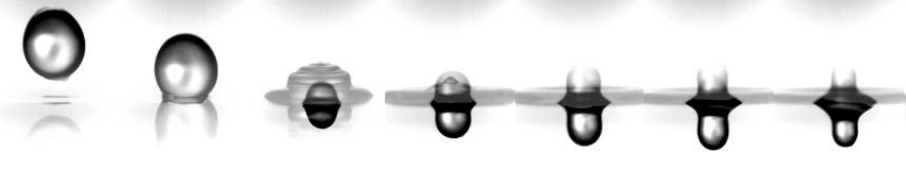
\includegraphics[width=1.0\linewidth]{figures/SiliconeOil2003_NoBreakUp2.png}}\qquad
        \subfloat[][Simulation: $V=0.3~m$ and $r=390~\mu m$]{
        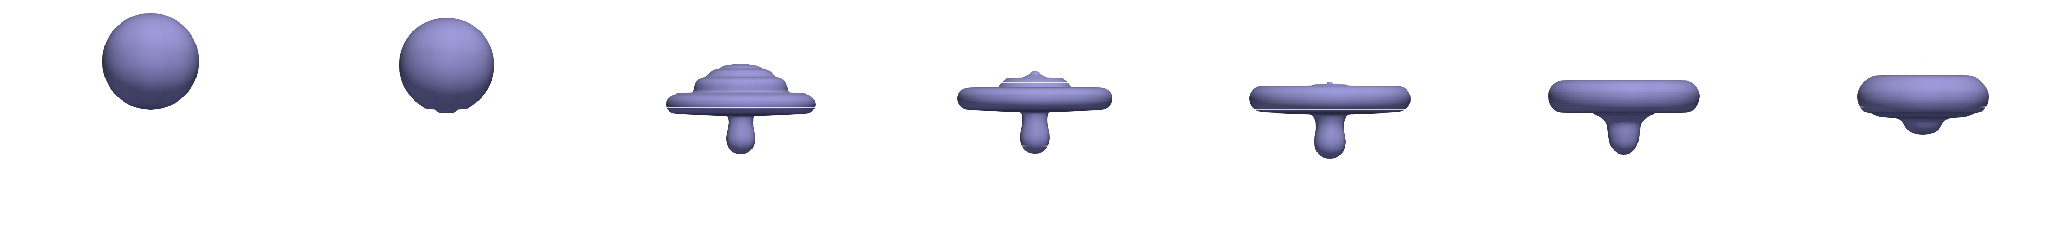
\includegraphics[width=1.0\linewidth]{figures/SiliconeOil2003_NoBreakUp_Simulation2.pdf}}\qquad
        \subfloat[][$V=0.7~m$ and $r=450~\mu m$]{
        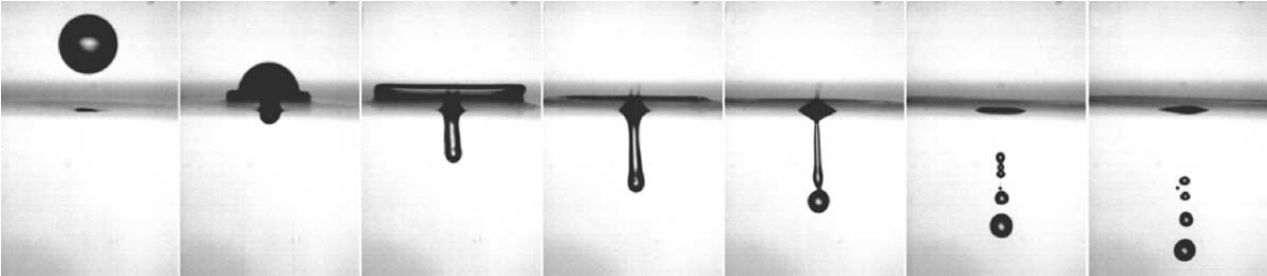
\includegraphics[width=1.0\linewidth]{figures/SiliconeOil2003_BreakUp.png}}\qquad
        \subfloat[][Simulation: $V=0.5~m$ and $r=450~\mu m$]{
        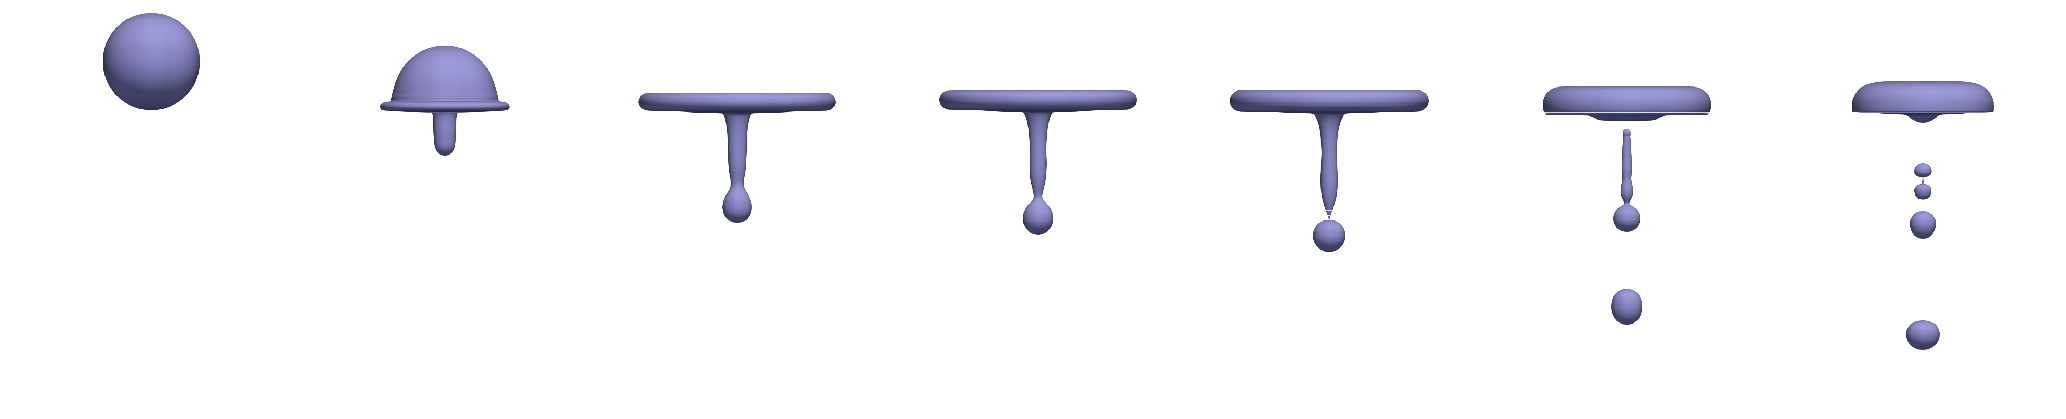
\includegraphics[width=1.0\linewidth]{figures/SiliconeOil2003_BreakUp_Simulation.png.pdf}}
        \caption{Silicone oil drop impacting a solid surface pierced with a small hole \cite{lorenceau2003drops}.}
        \label{ExpDrop2003}
    \end{figure}


\subsection{Results at the threshold velocity}

The threshold velocities obtained for each fluid and hole radius are presented in Table \ref{ThresholdVel}. In addition, we also included the theoretical speed at the regime {\it capillary-inertial} $V^{*} = 2\sqrt{\frac{\gamma}{\rho r}}$ using the silicone oil parameters for comparison. While the critical speed $V^*$ is consistently near $0.5$~m/s for the majority of the Newtonian cases, two distinct scenarios lead to a significant increase in the velocity required for droplet capture.
First, a geometric effect is observed: for the smallest hole radius ($r = 130~\mu m$), all fluids require a higher impact velocity to achieve breakup compared to the larger radii. This suggests that as the hole size decreases, the relative resistance to penetration increases, necessitating greater inertial force to overcome the capillary barrier.
Second, a fluid property effect is evident in the case of water. Regardless of the hole radius, water consistently exhibits the highest threshold velocities in the study. This behavior is attributed to high surface tension ($\gamma = 72$~mN/m) of the water, which is significantly greater than that of the other fluids considered. Since the viscosity of water is comparable to the other test fluids, this higher $V^*$ highlights the dominant role of capillary forces in stabilizing the droplet interface against breakup. 

It is important to note that these two effects—small hole geometry and high surface tension—act independently; however, their combination in the case of a water droplet impacting a $130~\mu m$ hole results in the highest critical velocity observed ($V^* = 1.0$~m/s).

\begin{table}[!h]
    \centering
    \caption{Threshold velocity $V^*$ (\si{\meter\per\second}) for different fluids and hole radii.}
    \label{ThresholdVel}
    \begin{tabular}{l *{4}{S[table-format=1.4]}}
        \toprule
        & \multicolumn{4}{c}{Hole radius $r$} \\
        \cmidrule(lr){2-5}
        Fluid & {\qty{130}{\micro\meter}} & {\qty{270}{\micro\meter}} & {\qty{390}{\micro\meter}} & {\qty{450}{\micro\meter}} \\
        \midrule
        Capillary-inertial regime~\cite{lorenceau2003drops} & 0.7161 & 0.4969 & 0.4134 & 0.3849 \\ 
        \midrule
        Silicone oil & 0.4750 & 0.3750 & 0.3375 & 0.3375 \\
        Acetone      & 0.6250 & 0.5000 & 0.4500 & 0.4375 \\
        Heptane      & 0.6250 & 0.5000 & 0.4500 & 0.4375 \\
        Ethanol      & 0.6250 & 0.5000 & 0.4500 & 0.4375 \\     
        Water        & 0.9750 & 0.7750 & 0.7000 & 0.6875 \\   
        \bottomrule
    \end{tabular}
\end{table}
    

%Using the threshold velocities from Table \ref{ThresholdVel}, we can characterize the competition between viscous, inertial, and capillary forces via the Reynolds ($Re = \frac{\rho V^* r}{\mu}$) and Weber ($We = \frac{\rho {V^*}^2 r}{\gamma}$) numbers. %Figure \ref{Exp} illustrates $We$ as a function of $Re$ at the threshold. Our numerical data are plotted alongside experimental values and the theoretical reference line $Re \sim \frac{We}{We - 1}$ proposed by Lorenceau \cite{lorenceau2003drops}.

Figure \ref{Exp} illustrates the correlation between the Weber $We=\frac{\rho {V^{*}}^{2} r}{\gamma}$ and Reynolds $Re=\frac{\rho V^{*} r}{\eta}$ numbers at the threshold where the droplet begins to {\it break up}. A comparison between our numerical results and the experimental data reveals strong agreement in all three regimes: viscous-inertial, intermediate ($5< Re <100$) and capillary-inertial ($Re>100$). In those regions, the numerical model accurately captures the transition to breakup predicted by the theoretical reference line $Re \sim \frac{aWe}{We-b}$, where $a$ and $b$ are constants determined by the numerical results. Table \ref{LSM} presents the values of $a$ and $b$ for all the four hole radii.

\begin{figure}[!h]
    \centering
    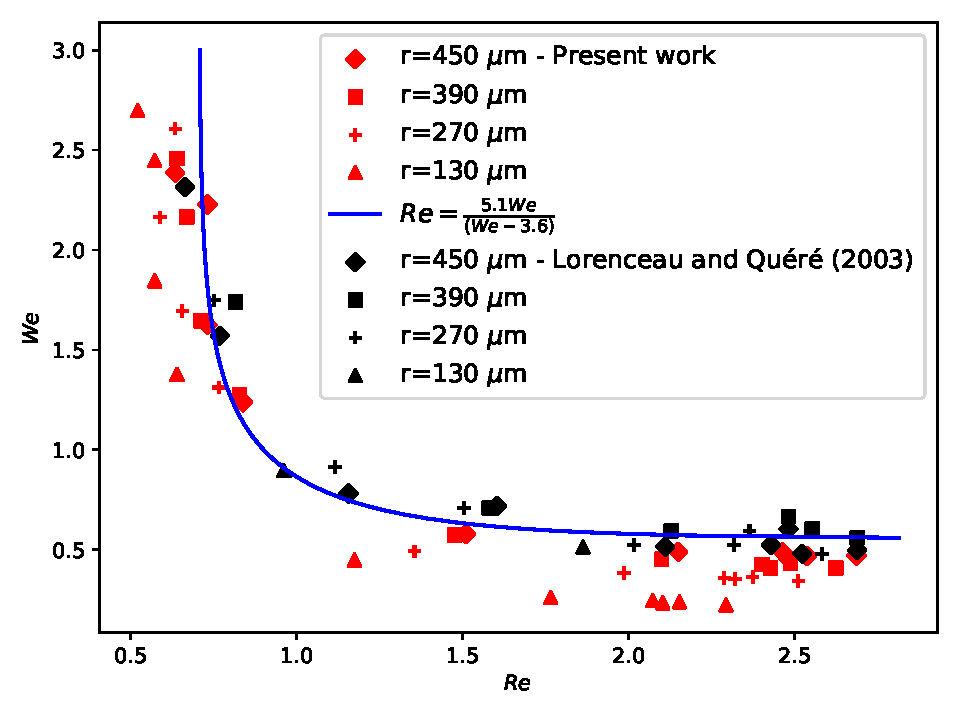
\includegraphics[width=0.8\linewidth]{figures/RexWe_ThresholdVelocities.pdf}
    \caption{Estimation of $Re$ and $We$ using the threshold velocities displayed in Table \ref{ThresholdVel}.}
    \label{Exp}
\end{figure}

\begin{table}[!h]
    \centering
    \caption{Parameters $a$ and $b$ fitted to the scaling relation $Re \sim \frac{a We}{We - b}$ using the Least Squares Method (LSM).}
    \label{LSM}
    \begin{tabular}{l *{2}{S[table-format=1.4]}}
        \toprule
        {Hole radius $r$} & {$a$} & {$b$} \\
        \midrule
        Lorenceau and Quéré \cite{lorenceau2003drops} & 5.1000 & 3.6000 \\
        \midrule
        \qty{450}{\micro\meter} & 4.6186 & 2.9225 \\ 
        \qty{390}{\micro\meter} & 4.3986 & 2.5836 \\ 
        \qty{270}{\micro\meter} & 4.2463 & 2.2147 \\ 
        \qty{130}{\micro\meter} & 3.4188 & 1.6772 \\ 
        \bottomrule
    \end{tabular}
\end{table}


Following the work of Lorenceau and Quéré \cite{lorenceau2003drops}, we present in Figure \ref{Capillary_Inertial} the relation between the threshold velocity and the capillary. In addition, we present in Table \ref{LSM2} the estimates of coefficients $\alpha_{0}$ and $\alpha_{1}$ of the expression $y = \alpha_{0}\left( \gamma / \rho r \right)^{\alpha_{1}}$.

\begin{figure}[!h]
    \centering
    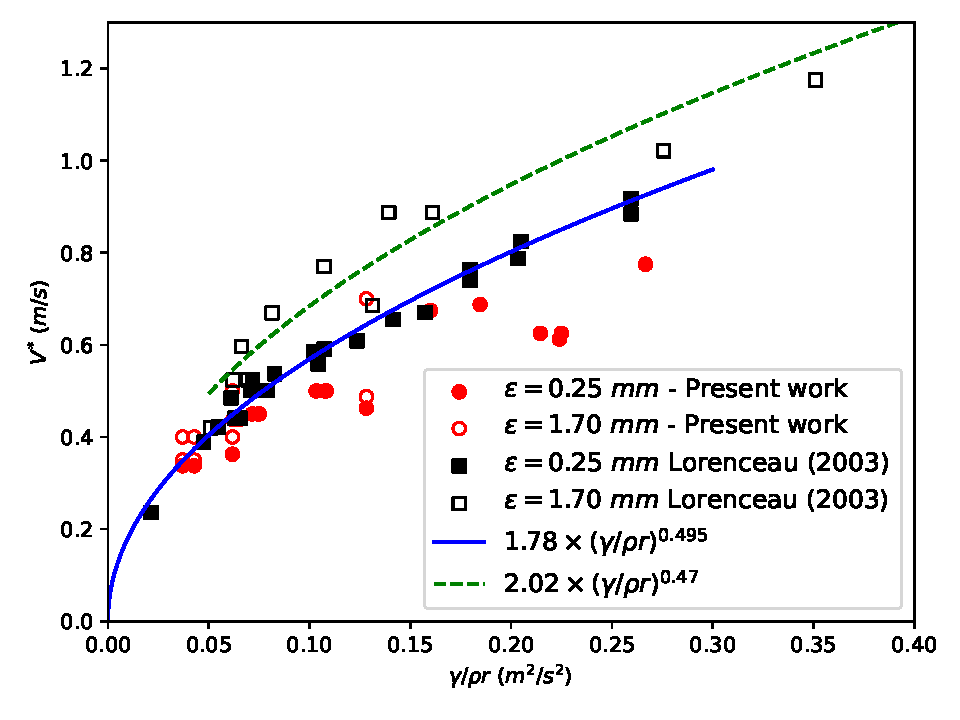
\includegraphics[width=0.8\linewidth]{figures/Capillary_Inertial.pdf}
    \caption{Relation between the threshold velocity $V^{*}$ and the capillary $\gamma / \rho r$. We also included the power law function with exponent 0.495 and coefficient of 1.78, as predicted in \cite{lorenceau2003drops}.}
    \label{Capillary_Inertial}
\end{figure}

\begin{table}[!h]
    \centering
    \caption{Parameters $\alpha_{0}$ and $\alpha_{1}$ fitted to the scaling relation $V^{*} \sim \alpha_{0}\left( \gamma / \rho r \right)^{\alpha_{1}}$ using the Least Squares Method (LSM).}
    \label{LSM2}
    \begin{tabular}{l *{2}{S[table-format=1.4]}}
        \toprule
        {Plate thickness $\epsilon$} & {$\alpha_{0}$} & {$\alpha_{1}$} \\
        \midrule
        $\epsilon=0.25$mm - Lorenceau and Quéré \cite{lorenceau2003drops} & 1.78 & 0.495 \\
        $\epsilon=1.70$mm - Lorenceau and Quéré \cite{lorenceau2003drops} & 2.02 & 0.470 \\
        \midrule
        $\epsilon=0.25$mm & 1.1839 & 0.3813 \\ 
        $\epsilon=1.70$mm & 1.2669 & 0.3769 \\         
        \bottomrule
    \end{tabular}
\end{table}

{\color{purple}
\begin{itemize}
    \item Resultados dos mapas de quebra da gota com diferentes shapes.
\end{itemize}
}

\subsection{Below the threshold velocity}
{\color{purple}
Aqui, vamos adicionar
\begin{itemize}
    \item Resultados do diâmetro máximo $D_{max}$ e comprimento máximo $H_{max}$.
\end{itemize}
}

\subsection{Above the threshold velocity}
{\color{purple}
Aqui, vamos adicionar
\begin{itemize}
    \item Resultados do tempo de quebra $t^{*} \times V$ ({\it time of pinch off}).
    \item Comprimento máximo $H_{max} \times V t_{R}$
\end{itemize}
}


%---------------------------------------------%
%---------------------------------------------%
%---------------------------------------------%
%---------------------------------------------%
%---------------------------------------------%
\section{Numerical results}\label{results}

This section presents a comparison of the numerical results for the flow simulation of droplets with different initial shapes impacting a surface pierced with a small hole. We define the ellipse reported by \cite{lorenceau2003drops} as a baseline and compare it against stretched oval shapes commonly observed in experimental settings \cite{Liu2021}, exploring how horizontal and vertical droplet stretching affects horizontal diameter, droplet elongation through the hole and threshold velocity.

We simulate silicone oil droplets with different viscosities ($\eta$), ranging between 0.5 and 50 $\si{\milli\pascal\second}$, based on the experimental data reported by \cite{lorenceau2003drops}. To investigate the importance of droplet shape, the elliptical shape used in the original work, with a droplet diameter of $D = 3.5$~mm, is compared with horizontally and vertically stretched droplets with the same total fluid volume but different aspect ratios ($Ar = \frac{(x_{max} - x_{min})}{(y_{max} - y_{min})}$). Additionally, the hole radius is varied across six values: $r = 130, 200, 270, 330, 390$ and $450~\mu m$, while the plate thickness is fixed at $\epsilon = 0.25$~mm. The physical and geometrical properties of these simulations (viscosity $\eta$, surface tension $\gamma$, density $\rho$, droplet aspect ratio $Ar$ and hole radius $r$) are summarized in Table \ref{NewtFluidsShapes}. 

\begin{table}[!ht]
\centering
\caption{Physical and geometrical properties of the fluids used in the simulations: dynamic viscosity $\eta$, surface tension $\gamma$, density $\rho$, droplet aspect ratio $Ar$ and hole radius $r$.}
\label{NewtFluidsShapes}
\begin{tabular}{lc}
\toprule
\multicolumn{2}{c}{\textbf{Fluid properties}} \
\midrule
Fluid & Silicone oil \
Dynamic viscosity, $\eta$ (\si{\milli\pascal\second}) & 0.5, 5, 50 \
Surface tension, $\gamma$ (\si{\milli\newton\per\meter}) & 16 \
Density, $\rho$ (\si{\kilogram\per\cubic\meter}) & 960 \
\midrule
\multicolumn{2}{c}{\textbf{Droplet geometries}} \
\midrule
Shape & Aspect ratio, $Ar$ \
Ellipse & 1.00 \
H-Oval & 1.87 \
V-Oval & 0.56 \
H-Stretch & 3.74 \
V-Stretch & 0.30 \
\midrule
\multicolumn{2}{c}{\textbf{Hole radius}} \
\midrule
\multicolumn{2}{c}{$r$ ($\si{\micro\meter}$)} \
\multicolumn{2}{c}{130, 200, 270, 330, 390, 450} \
\bottomrule
\end{tabular}
\end{table}

The threshold velocities $V^*$ obtained from the numerical comparisons may be subject to small uncertainties due to the finite resolution of the impact velocities considered. Furthermore, direct comparisons between different viscosities are not appropriate, as the impact velocity ranges considered differ depending on the fluid viscosity, with higher viscosities requiring higher impact velocities to capture the transition between breakup and no breakup regimes. Instead, the analysis focuses on identifying trends in the effect of droplet shape that persist across different fluid parameters and assessing their consistency with the findings of the original study, which considered only elliptical droplets. 

\subsection{Results at the threshold velocity}

The threshold velocities obtained for each fluid, shape and hole radius are presented in Table \ref{ThresholdVelShape}. Two geometric effects are observed. First, consistent with the previously reproduced experimental cases, the dependence on hole radius is also observed across the different droplet shapes, with smaller hole radii leading to considerably higher threshold velocities. Second, horizontally stretched droplets exhibit a greater propensity for breakup, whereas vertically stretched droplets exhibit a greater resistance. Horizontally stretched droplets may spread more readily along the surface after penetration, promoting further deformation and destabilization, while vertically stretched droplets may retain an elongation along the direction of penetration, delaying breakup.

\begin{table}[!h]
    \centering
    \caption{Threshold velocity $V^*$ (\si{\meter\per\second}) for different fluids, shapes and hole radii.}
    \label{ThresholdVelShape}
    \begin{tabular}{l *{4}{S[table-format=1.4]}}
        \toprule
        & \multicolumn{6}{c}{Hole radius $r$} \\
        \cmidrule(lr){3-8}
        Viscosity (\si{\milli\pascal\second}) & Shape & {\qty{130}{\micro\meter}} & {\qty{200}{\micro\meter}} & {\qty{270}{\micro\meter}} & {\qty{330}{\micro\meter}} & {\qty{390}{\micro\meter}} & {\qty{450}{\micro\meter}} \\
        \midrule
        0.5 & Ellipse   & 0.5500 & 0.4375 & 0.4375 & 0.4375 & 0.4375 & 0.3250 \\
        0.5 & H-Oval    & 0.4375 & 0.4375 & 0.3250 & 0.3250 & 0.3250 & 0.3250 \\
        0.5 & V-Oval    & 0.6625 & 0.5500 & 0.4375 & 0.4375 & 0.4375 & 0.3250 \\
        0.5 & H-Stretch & 0.4375 & 0.3250 & 0.3250 & 0.3250 & 0.3250 & 0.3250 \\
        0.5 & V-Stretch & 0.6625 & 0.5500 & 0.4375 & 0.4375 & 0.4375 & 0.4375 \\

        5   & Ellipse   & 0.7063 & 0.4938 & 0.4938 & 0.4938 & 0.3875 & 0.3875 \\
        5   & H-Oval    & 0.4938 & 0.4938 & 0.3875 & 0.3875 & 0.3875 & 0.3875 \\
        5   & V-Oval    & 0.8125 & 0.6000 & 0.4938 & 0.4938 & 0.4938 & 0.3875 \\
        5   & H-Stretch & 0.4938 & 0.3875 & 0.3875 & 0.3875 & 0.3875 & 0.3875 \\
        5   & V-Stretch & 0.9188 & 0.7063 & 0.6000 & 0.4938 & 0.4938 & 0.4938 \\
        
        50  & Ellipse   & 1.7500 & 1.2500 & 1.0000 & 1.0000 & 1.0000 & 0.7500 \\
        50  & H-Oval    & 1.5000 & 1.0000 & 1.0000 & 1.0000 & 0.7500 & 0.7500 \\
        50  & V-Oval    & 2.0000 & 1.5000 & 1.2500 & 1.0000 & 1.0000 & 1.0000 \\
        50  & H-Stretch & 1.2500 & 1.0000 & 1.0000 & 0.7500 & 0.7500 & 0.7500 \\
        50  & V-Stretch & 2.5000 & 1.7500 & 1.2500 & 1.2500 & 1.0000 & 1.0000 \\
        
        \bottomrule
    \end{tabular}
\end{table}

Figure \ref{fig:grafico_Re_vs_We_shapes} illustrates the correlation between the Weber $We=\frac{\rho {V^{*}}^{2} r}{\gamma}$ and Reynolds $Re=\frac{\rho V^{*} r}{\eta}$ numbers at the threshold. The solid curves for each shape are defined by the scaling relation $Re \sim \frac{a We}{We - b} + c$, with parameters $a$, $b$ and $c$ fitted using the Least Squares Method (LSM). Results show that, other than scaling differences, initial droplet shape does not significantly affect the three regimes (viscous-inertial, intermediate, and capillary-inertial) defined in the original work.

\begin{figure}[!h]
    \centering
    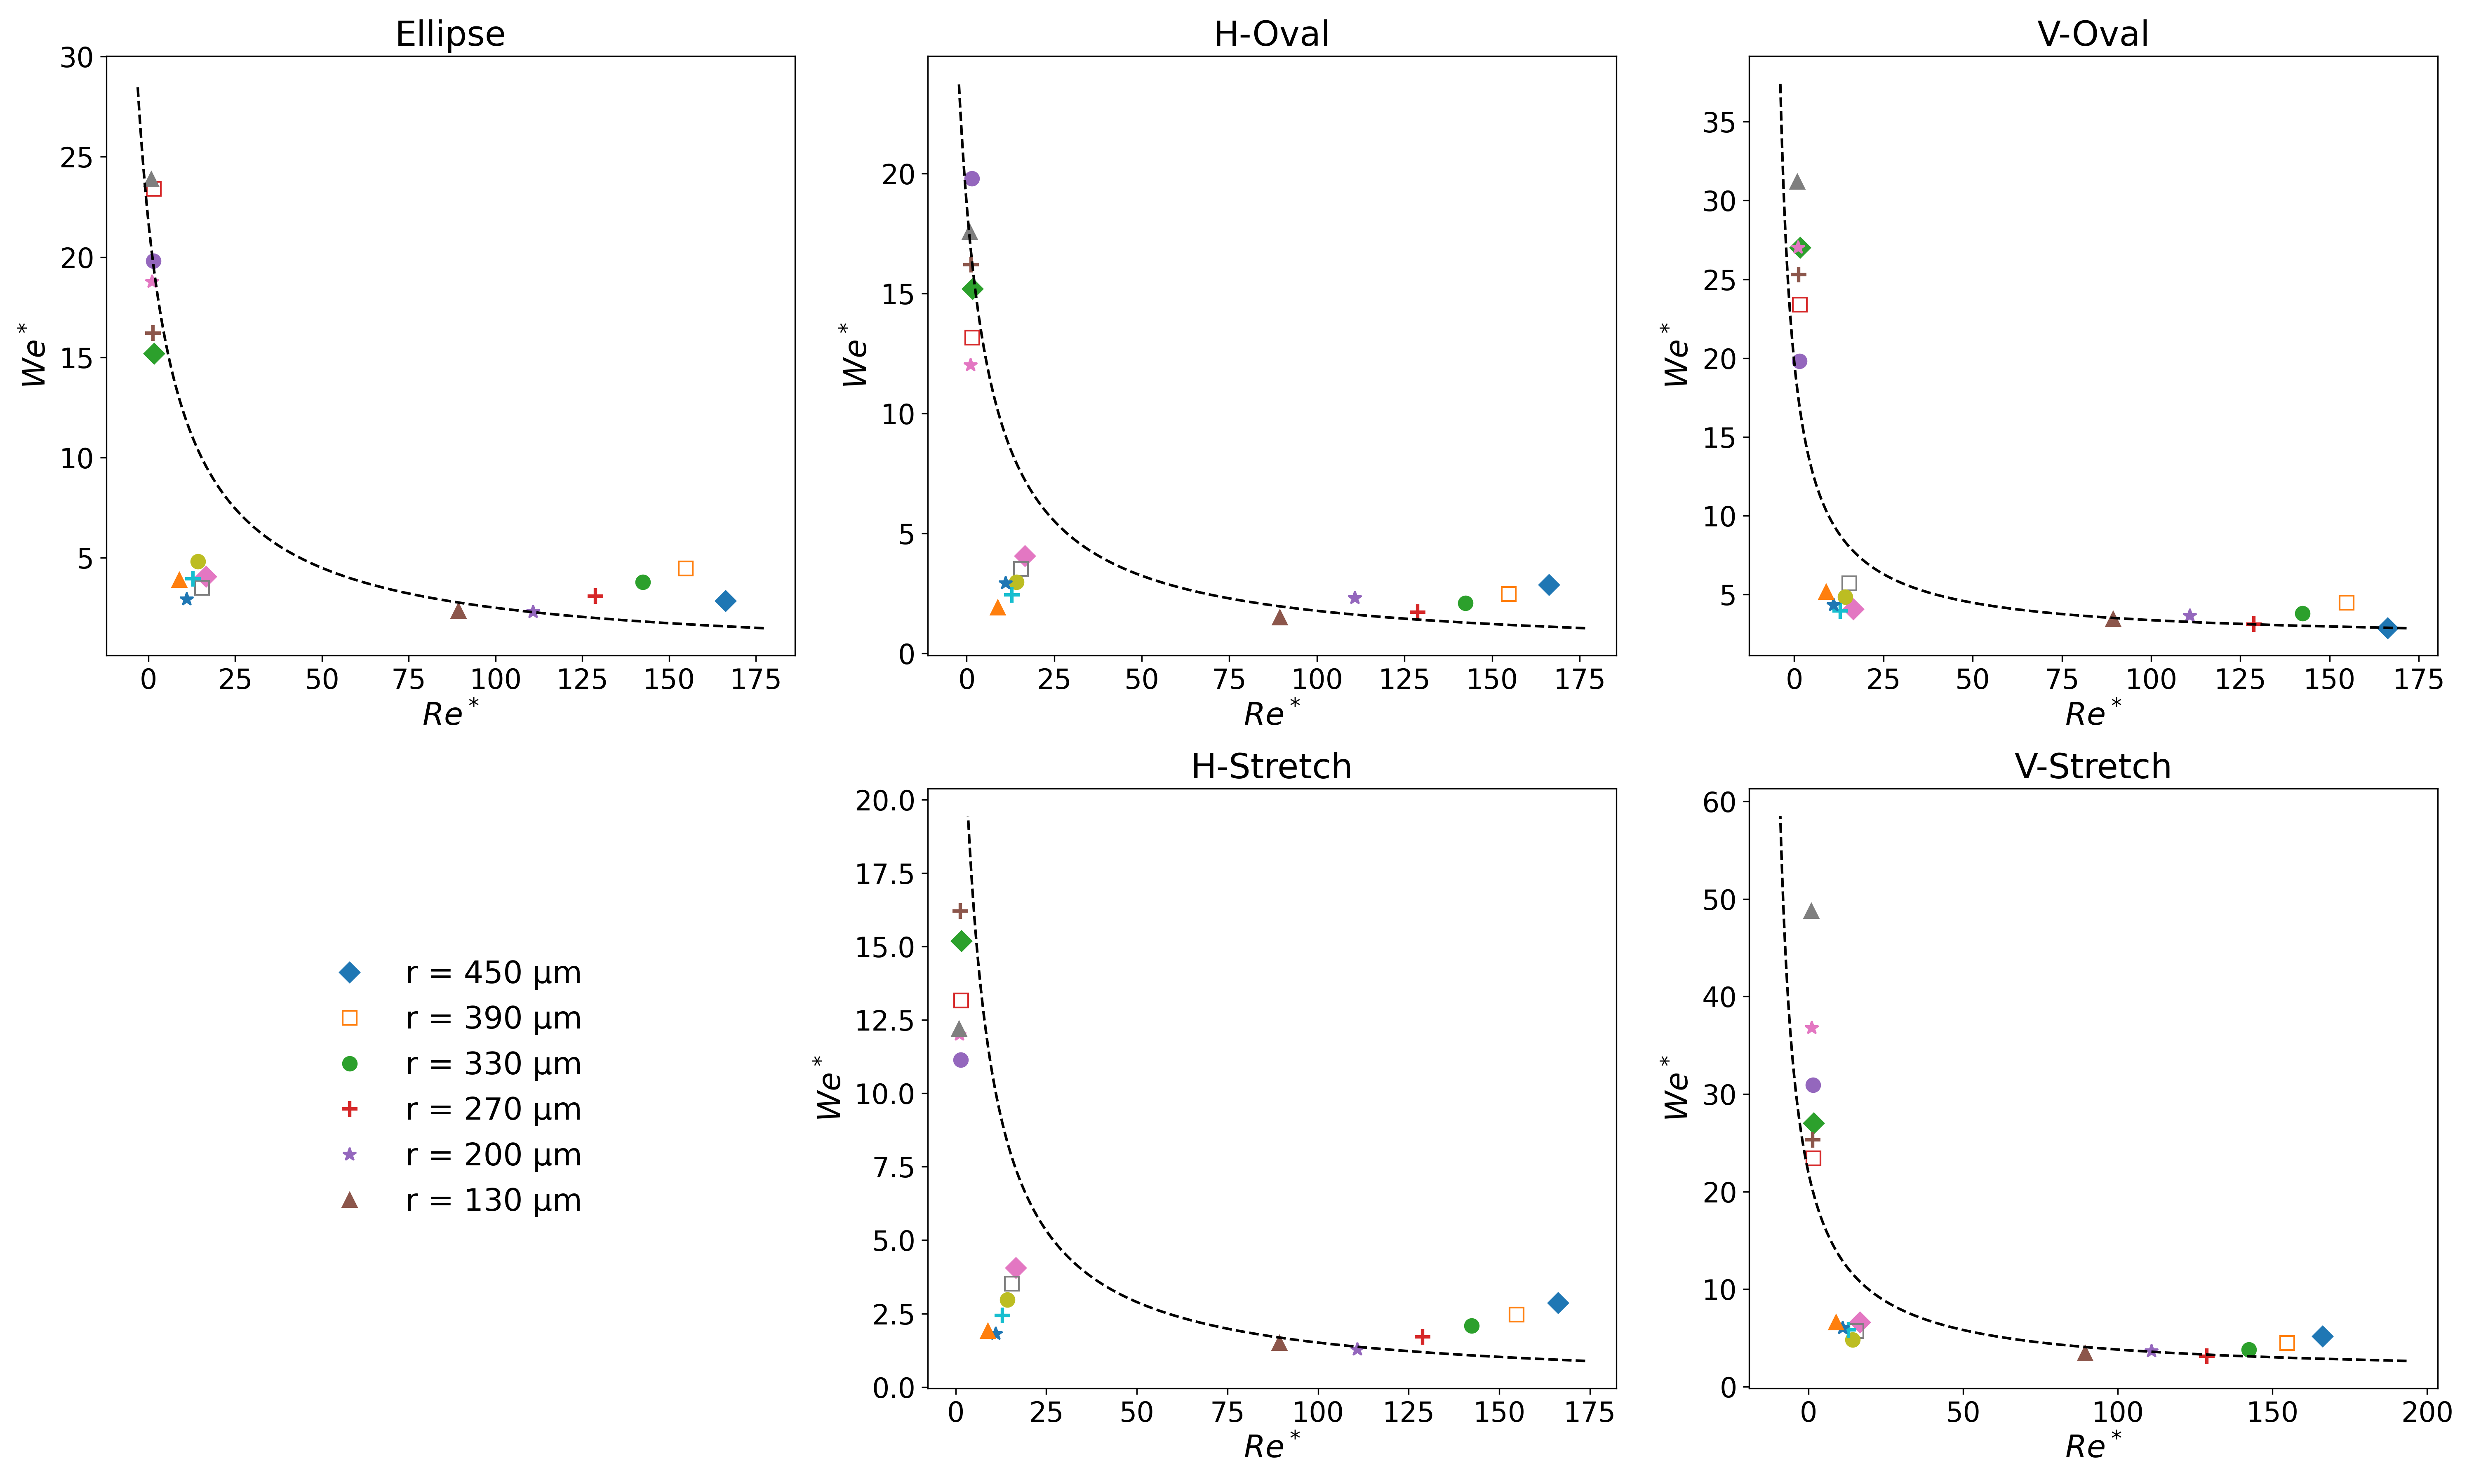
\includegraphics[width=0.8\linewidth]{figures/shape/grafico_Re_vs_We_shapes}
    \caption{Estimation of $Re$ and $We$ using the threshold velocities displayed in Table \ref{ThresholdVelShape}.}
    \label{fig:grafico_Re_vs_We_shapes}
\end{figure}

A comparison of breakup regimes and threshold velocities for different droplet shapes is presented in Figure \ref{fig:classificacao_shapes}. The bar chart highlights the effect of droplet shape on the critical breakup velocity, showing that horizontal stretching consistently lowers the breakup threshold across all viscosities, whereas vertical stretching increases it.

\begin{figure}[!h]
    \centering
    \begin{subfigure}[b]{0.32\textwidth}
        \centering
        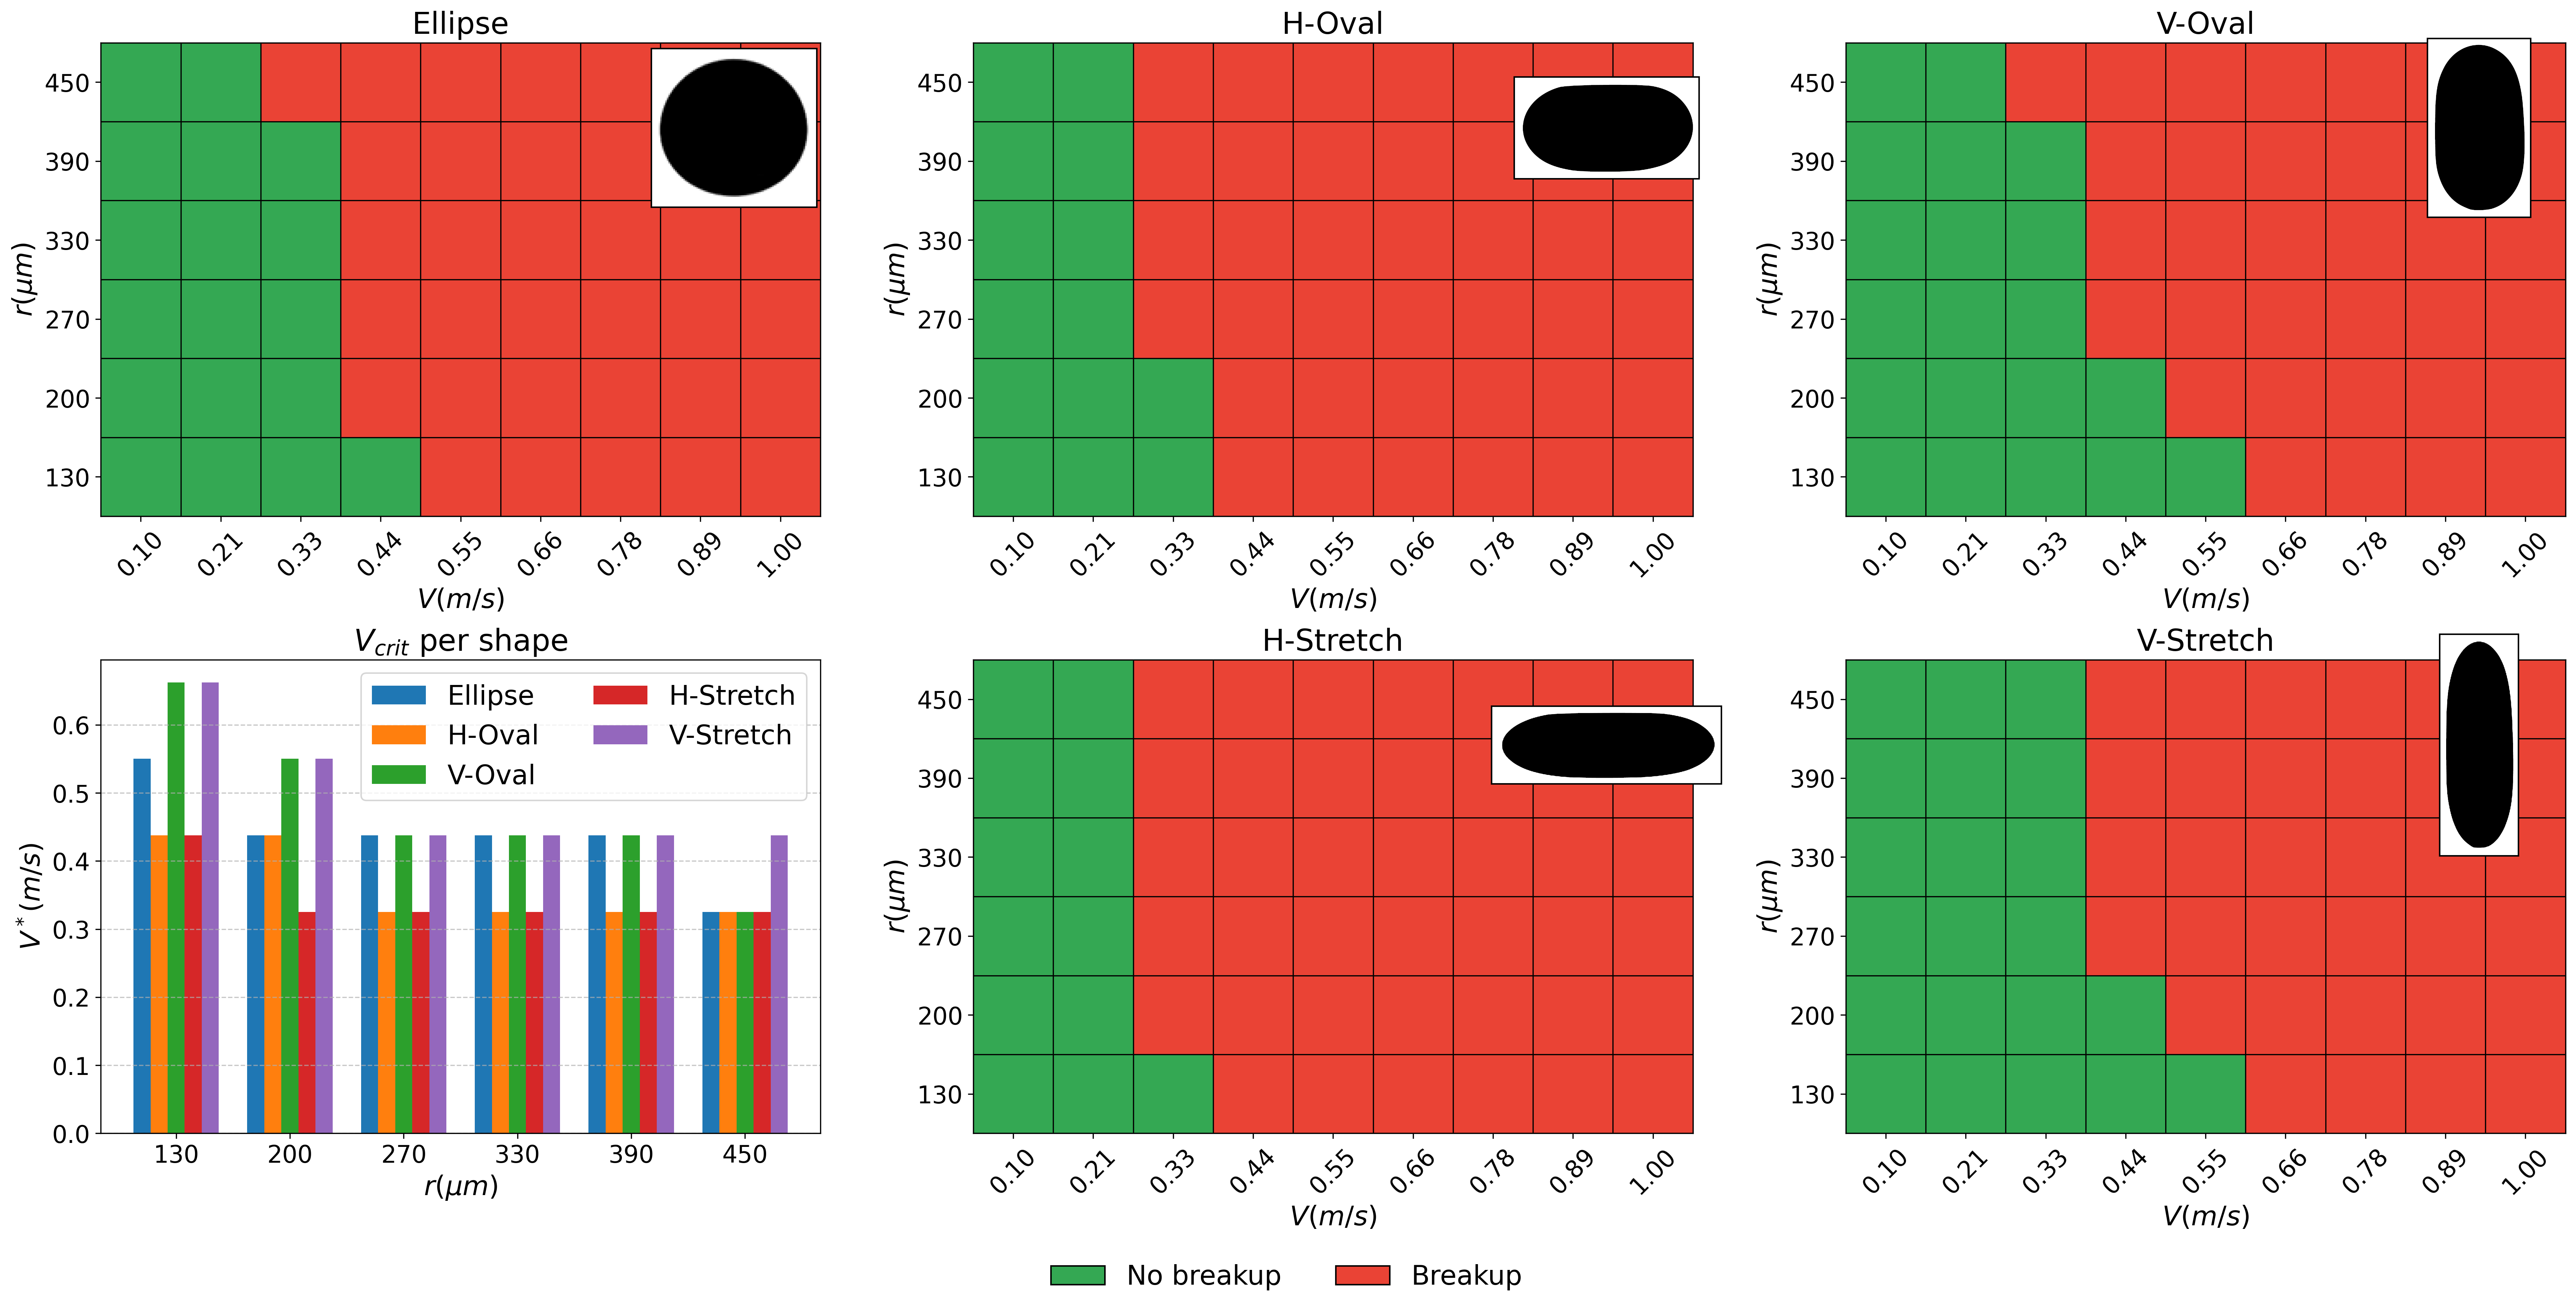
\includegraphics[width=\linewidth]{figures/shape/visc0.0005/grafico3_classificacao_com_imagens_shapes_dados_0.0005}
        \caption{Breakup regime maps for μ = 0.5 \si{\milli\pascal\second}.}
        \label{fig:classificacao_shapes_0.0005}
    \end{subfigure}
    \hfill
    \begin{subfigure}[b]{0.32\textwidth}
        \centering
        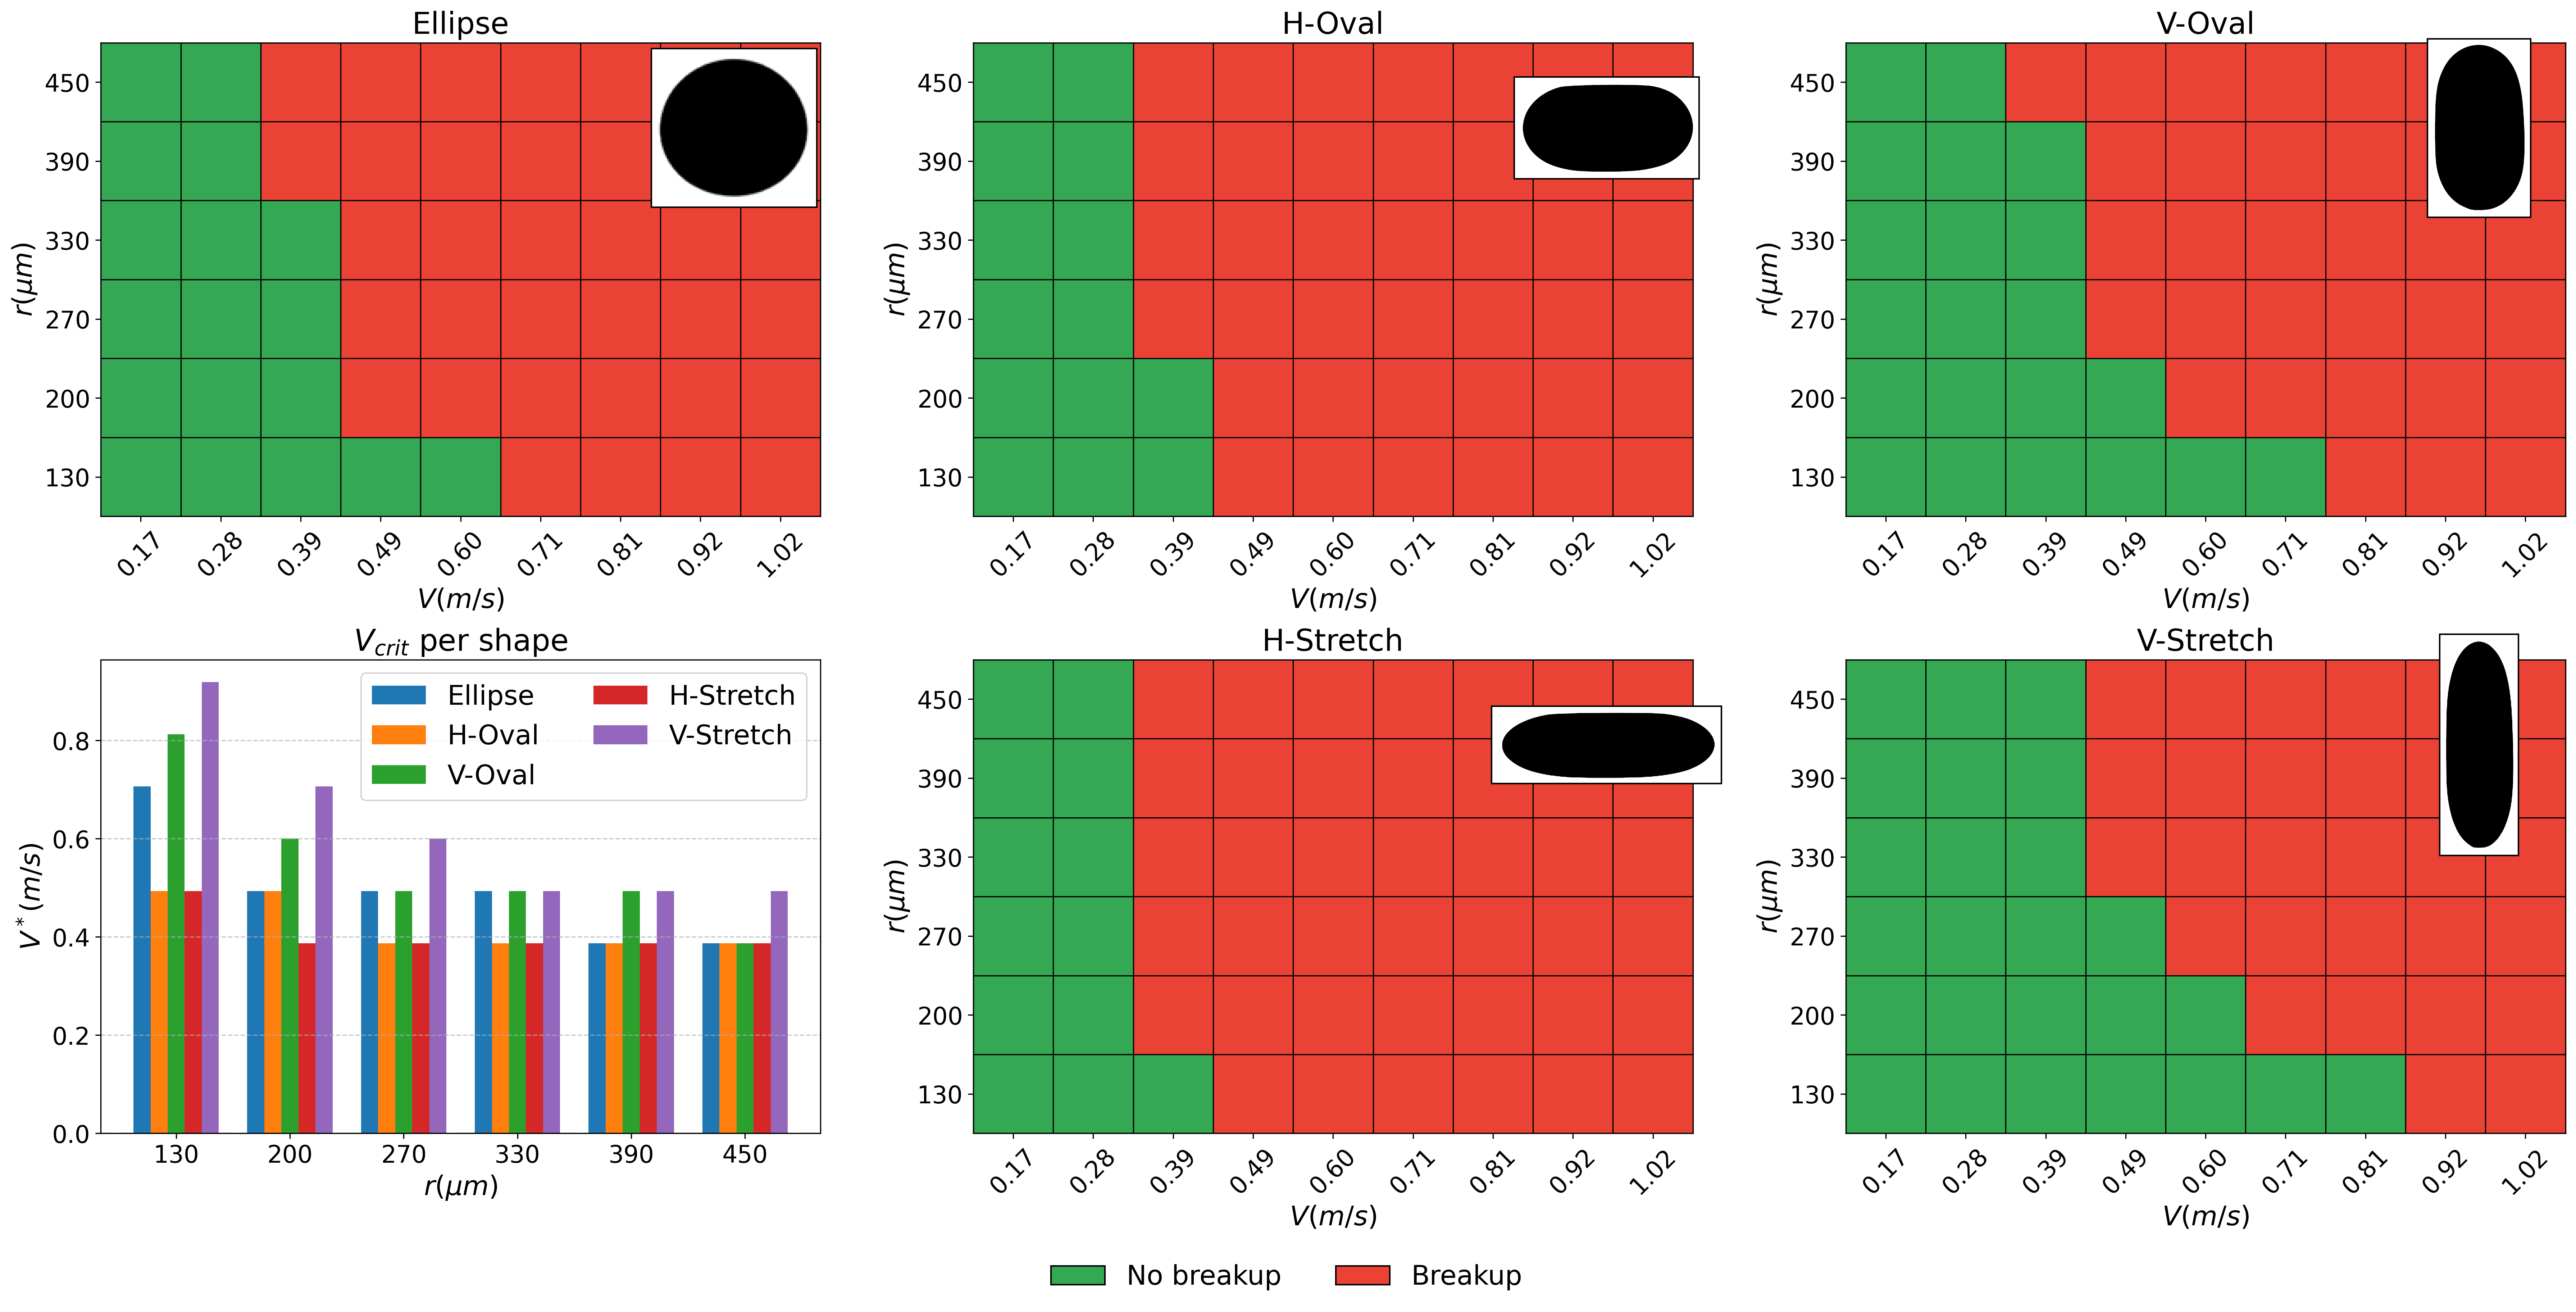
\includegraphics[width=\linewidth]{figures/shape/visc0.005/grafico3_classificacao_com_imagens_shapes_dados_0.005}
        \caption{Breakup regime maps for μ = 5 \si{\milli\pascal\second}.}
        \label{fig:classificacao_shapes_0.005}
    \end{subfigure}
    \hfill
    \begin{subfigure}[b]{0.32\textwidth}
        \centering
        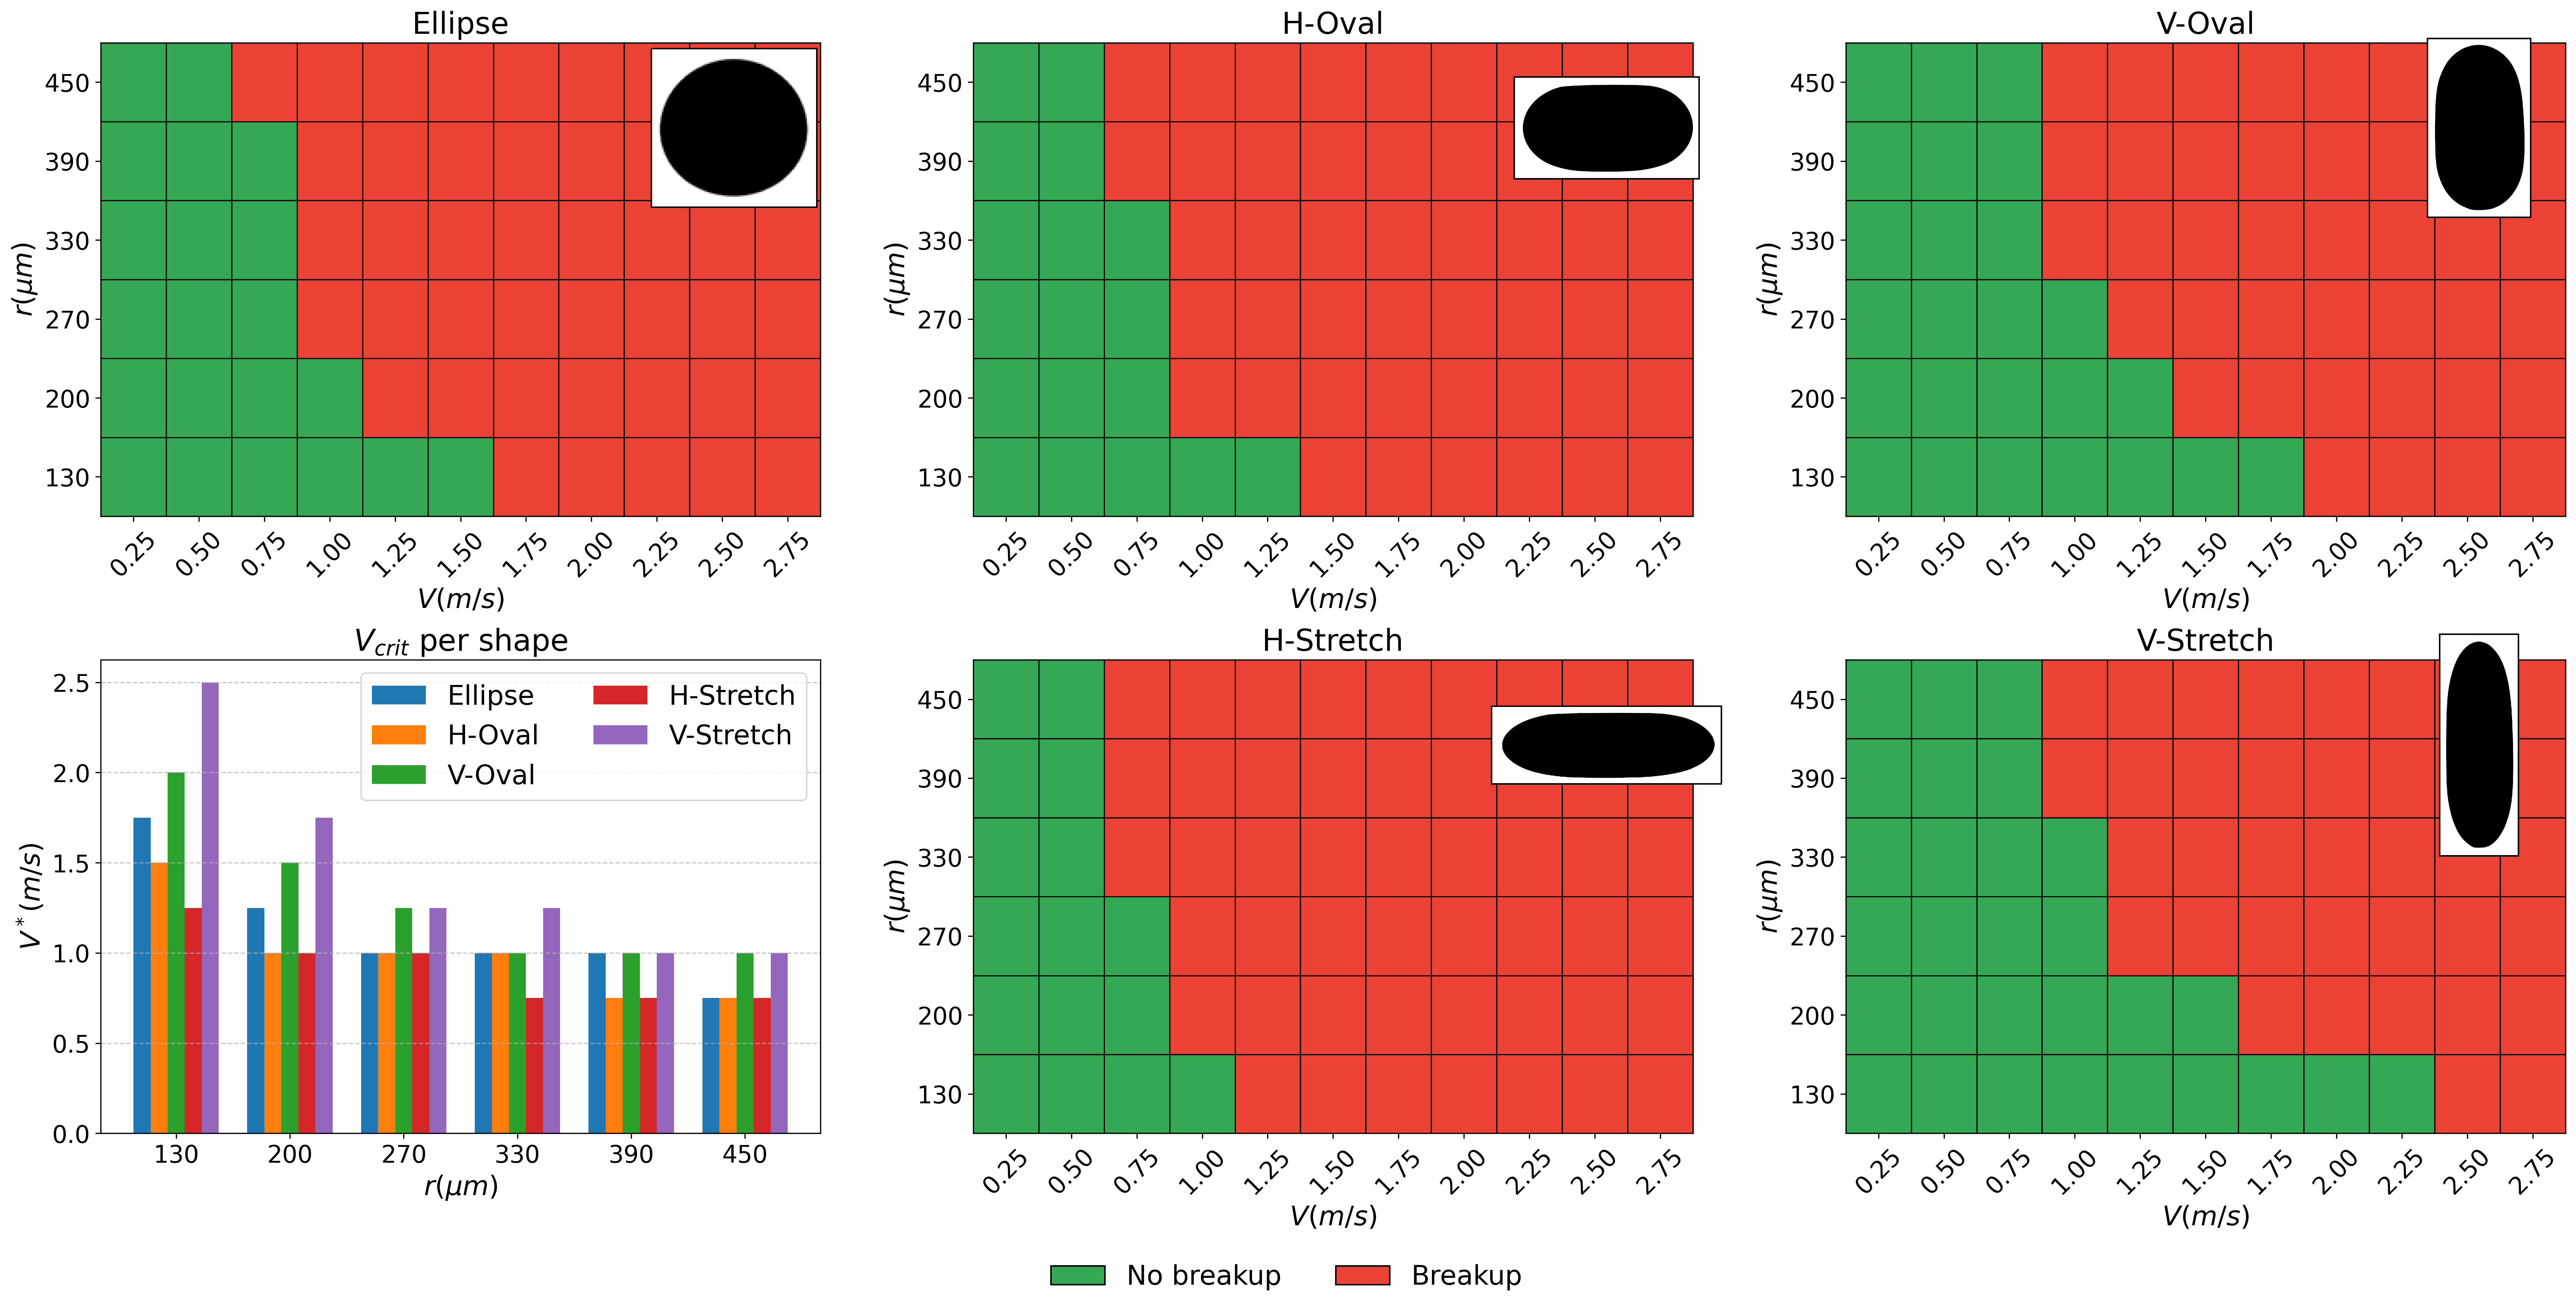
\includegraphics[width=\linewidth]{figures/shape/visc0.05/grafico3_classificacao_com_imagens_shapes_dados_0.05}
        \caption{Breakup regime maps for μ = 50 \si{\milli\pascal\second}.}
        \label{fig:classificacao_shapes_0.05}
    \end{subfigure}
    \caption{Breakup regime maps and critical velocity comparison for different droplet shapes and viscosities. Red and green represent breakup and no breakup regimes, respectively.}
    \label{fig:classificacao_shapes}
\end{figure}

\subsection{Droplet deformation}

Figure \ref{fig:diametro_vs_tempo} presents the temporal evolution of the horizontal droplet diameter ($D_t$) at selected impact velocities for the different droplet shapes, hole radii and viscosities explored. The same trends are also observed at other velocity variations.

The results show that vertically stretched droplets generally exhibit more oscillations in $D_t$. This behavior may be related to their greater initial deformations, which leads to more pronounced shape relaxations and subsequent oscillations driven by inertia and surface tension.

Another notable feature is that Horizontally stretched droplets generally reach their maximum horizontal diameter earlier than other shapes. However, this does not necessarily imply a larger maximum diameter than that of the other shapes, as discussed in a subsequent analysis.

As viscosity increases, the temporal evolution of the horizontal diameter becomes smoother, with fewer oscillations. Additionally, the differences between curves corresponding to different hole radii and initial droplet shapes tend to diminish. This suggests that droplet spreading dynamics on the pierced surface become less sensitive to hole radius and initial shape with higher viscosities.

Finally, the temporal evolution of $D_t$ does not seem to be directly determined by whether breakup occurs. For the selected impact velocities, different hole radii can lead to either breakup or no breakup, without a consistent correspondence between these regimes and the diameter curves. For example, in the elliptical shape, breakup occurs only for the largest hole radius $r = 450~\mu m$, yet the oscillation patterns differ considerably among the curves associated with the other radii. This result indicate that the evolution of the horizontal diameter is insufficient to characterize the penetration outcome.

%----------------------------------------------------%
%----------------------------------------------------%
%----------------------------------------------------%
\begin{figure}[!h]
    \centering
    \begin{subfigure}[b]{0.32\textwidth}
        \centering
        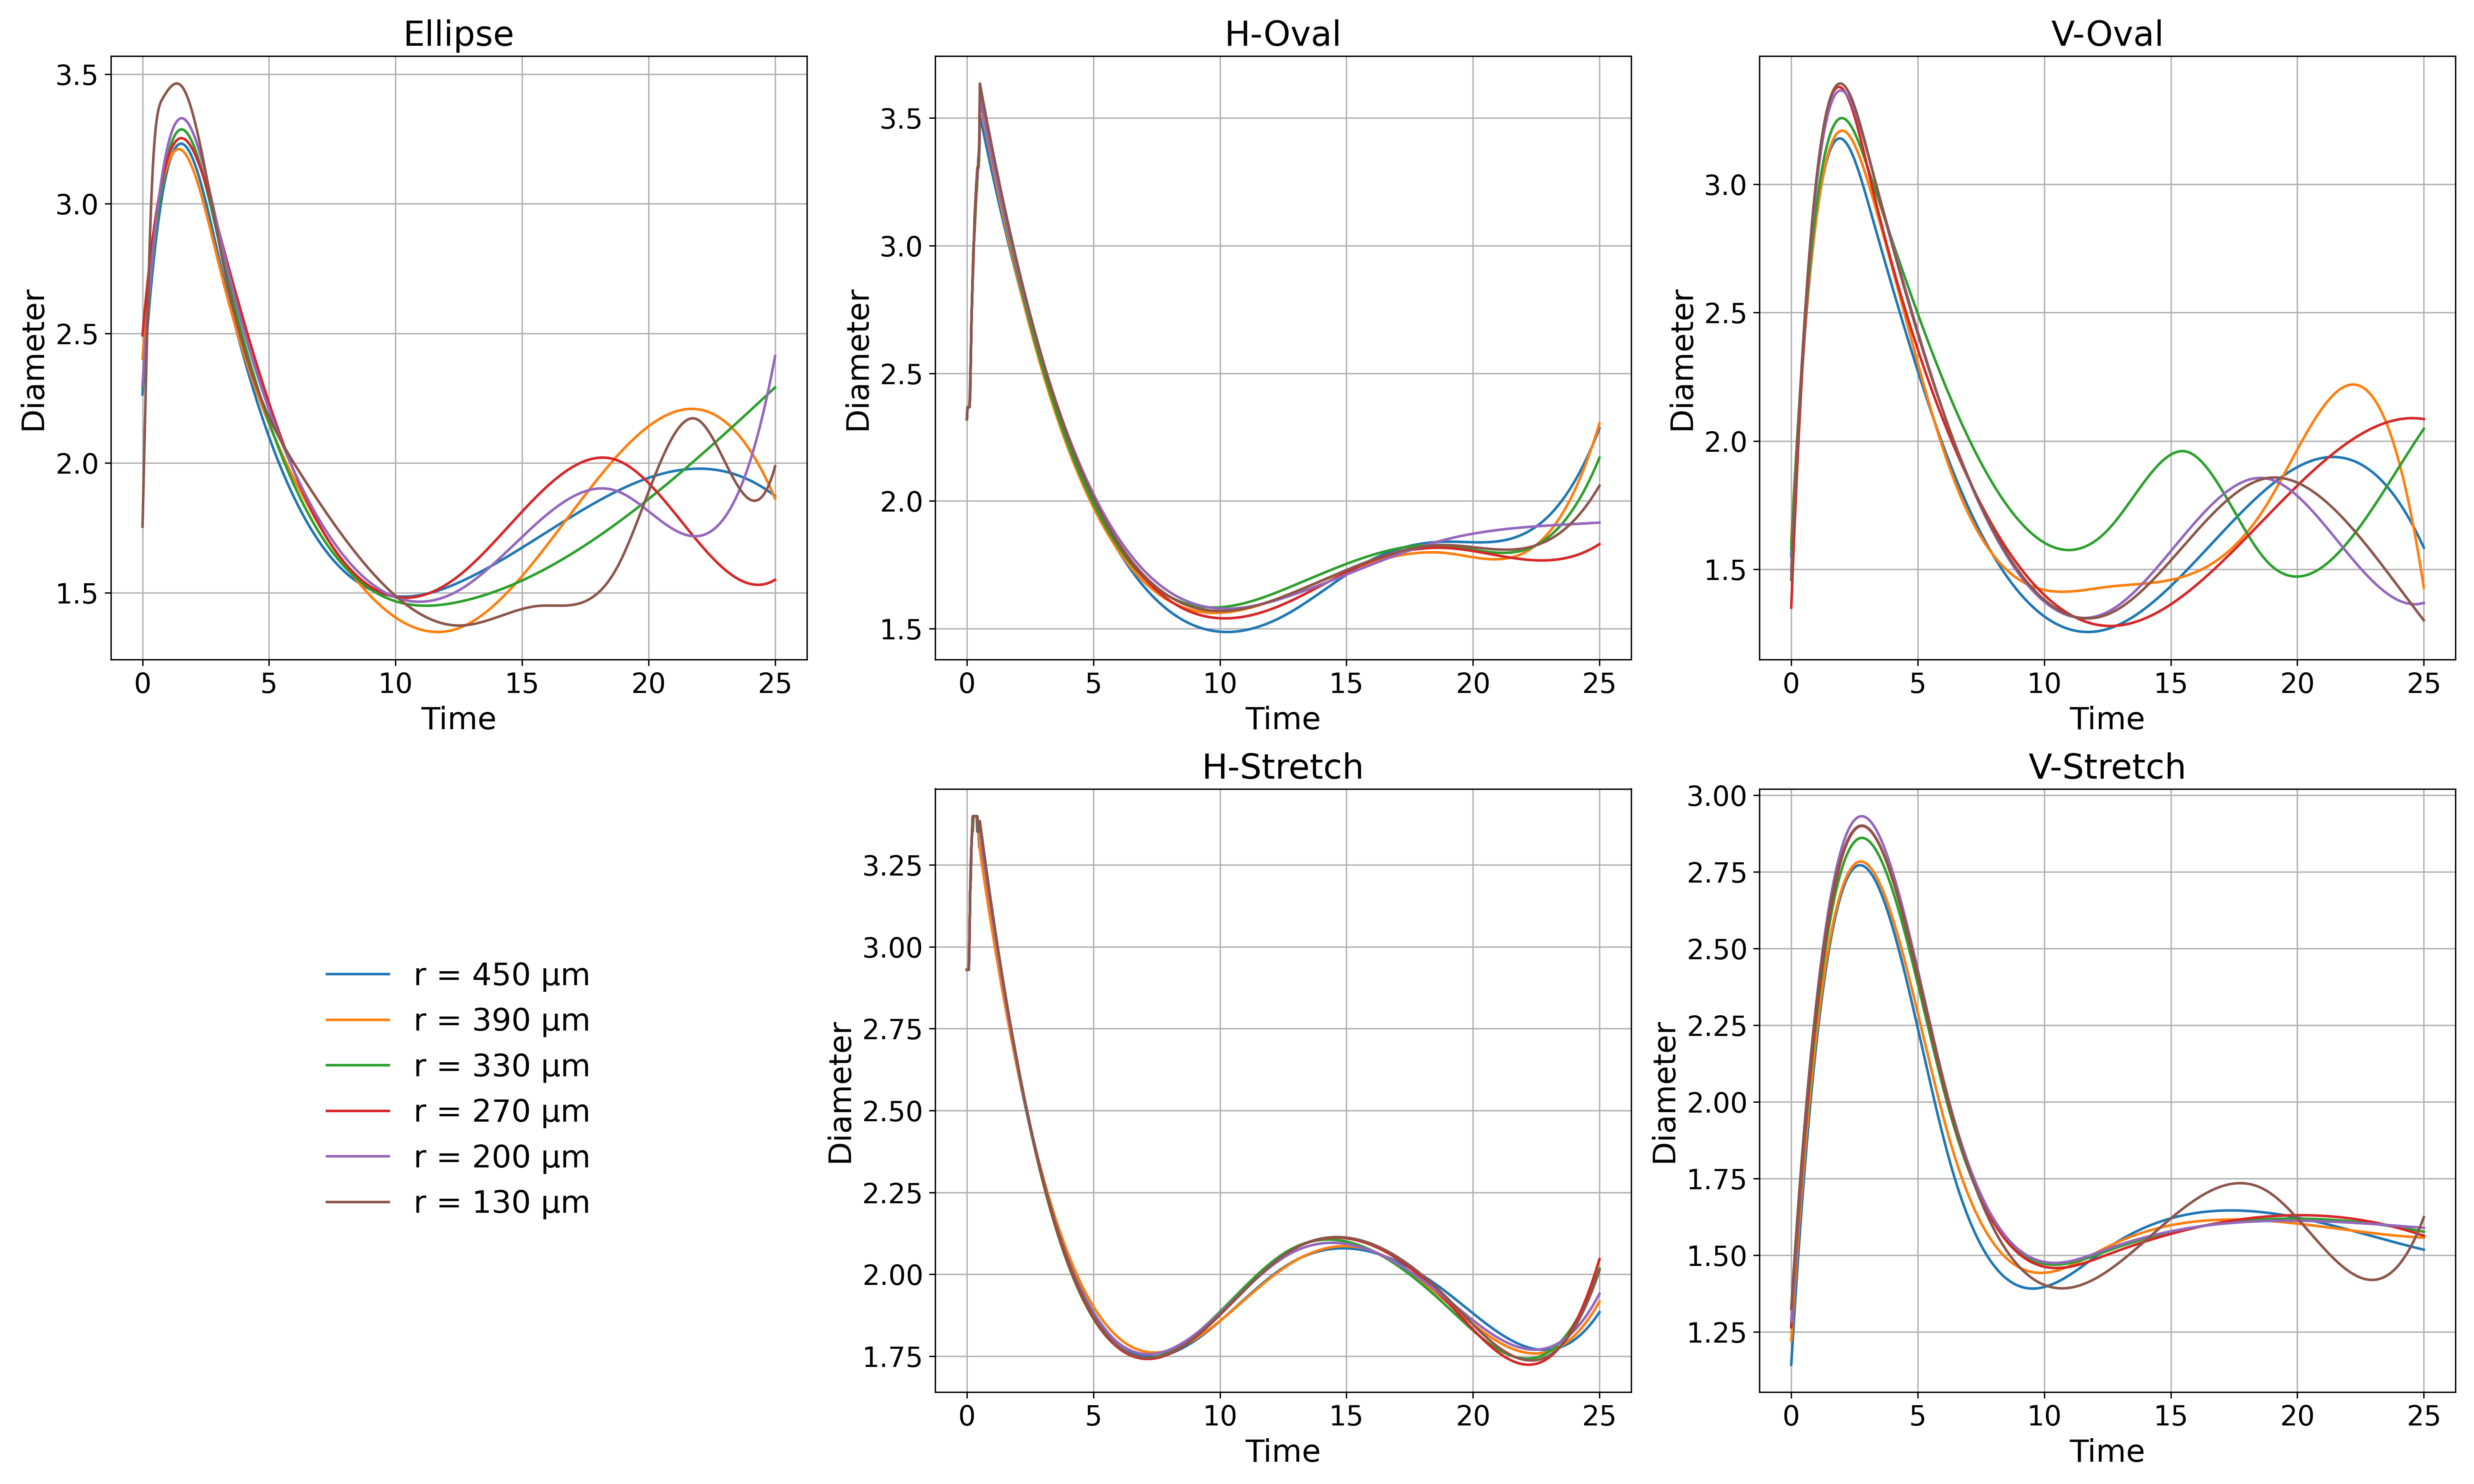
\includegraphics[width=\linewidth]{figures/shape/visc0.0005/grafico6_diametro_vs_tempo_dados_0.0005}
        \caption{Horizontal diameter at $V = 0.325~m/s$ and $\mu = 0.5$ \si{\milli\pascal\second}.}
        \label{fig:diametro_vs_tempo_0.0005}
    \end{subfigure}
    \hfill
    \begin{subfigure}[b]{0.32\textwidth}
        \centering
        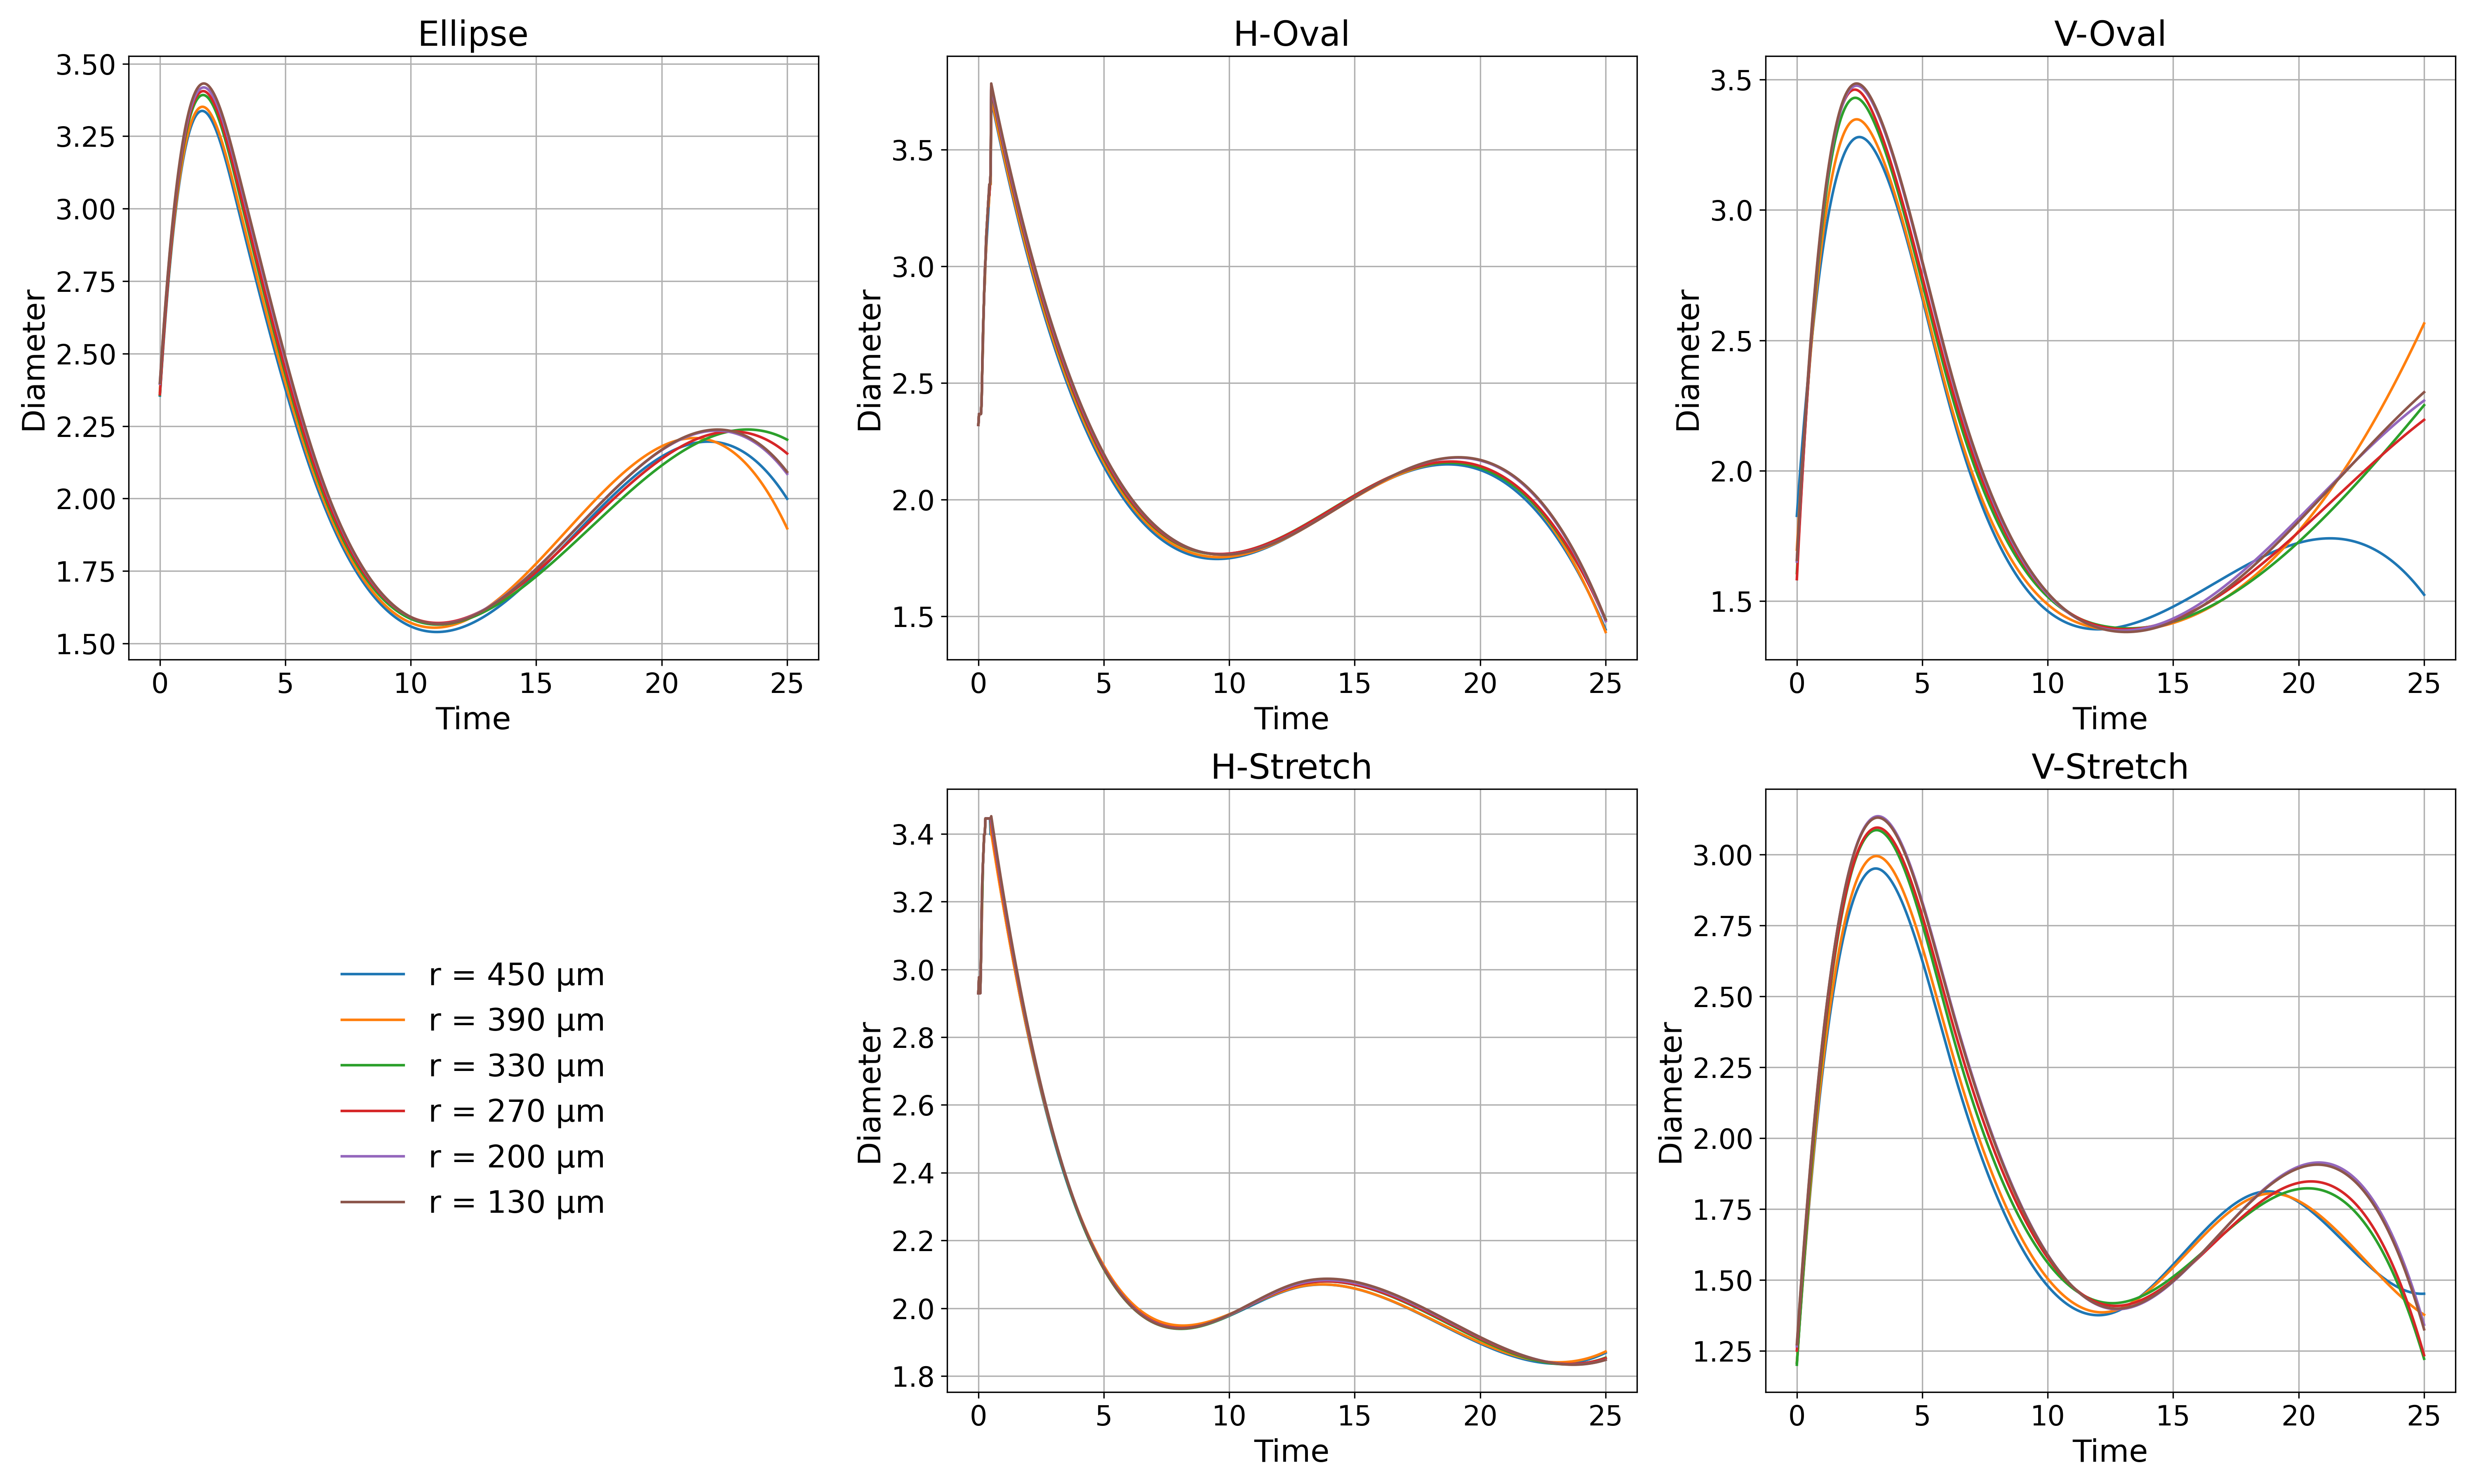
\includegraphics[width=\linewidth]{figures/shape/visc0.005/grafico6_diametro_vs_tempo_dados_0.005}
        \caption{Horizontal diameter at $V = 0.3875~m/s$ and $\mu = 5$ \si{\milli\pascal\second}.}
        \label{fig:diametro_vs_tempo_0.005}
    \end{subfigure}
    \hfill
    \begin{subfigure}[b]{0.32\textwidth}
        \centering
        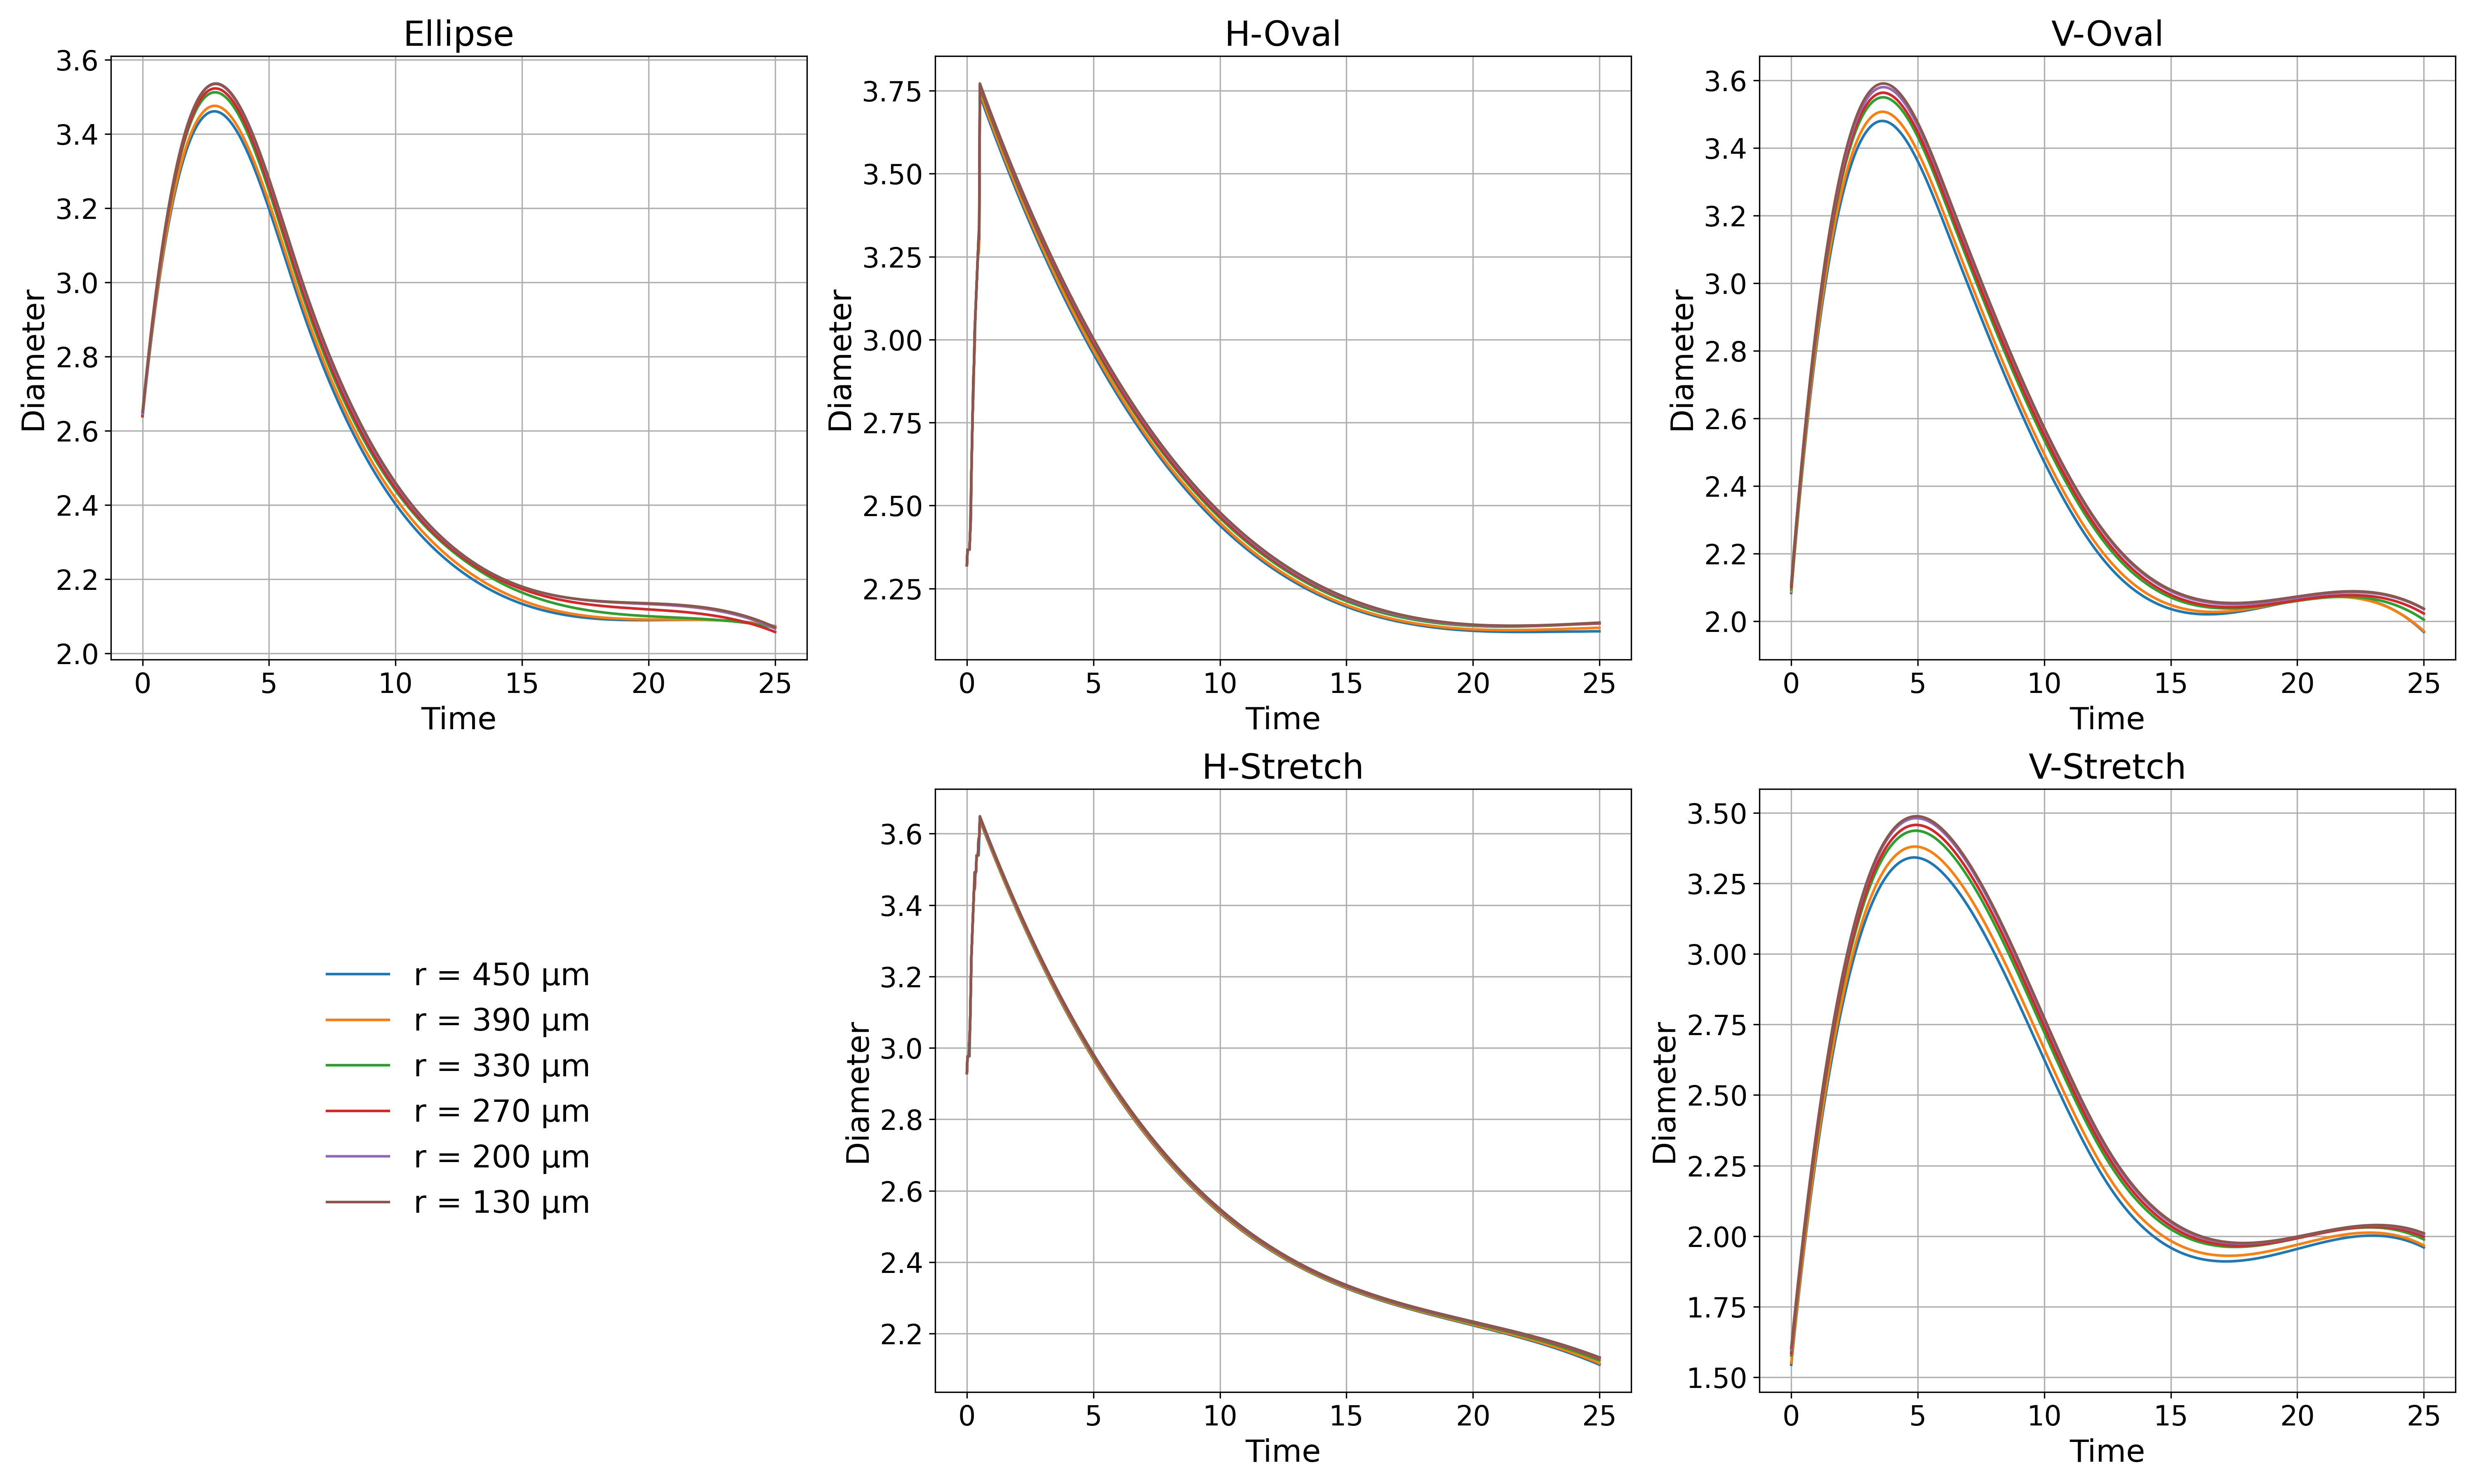
\includegraphics[width=\linewidth]{figures/shape/visc0.05/grafico6_diametro_vs_tempo_dados_0.05}
        \caption{Horizontal diameter at $V = 0.75~m/s$ and $\mu = 50$ \si{\milli\pascal\second}.}
        \label{fig:diametro_vs_tempo_0.05}
    \end{subfigure}
    \caption{Temporal evolution of the horizontal droplet diameter ($D_t$) for the five initial droplet shapes and six hole radii at selected impact velocities for viscosities of (a) 0.5, (b) 5 and (c) 50 \si{\milli\pascal\second}.}
    \label{fig:diametro_vs_tempo}
\end{figure}

Figure \ref{fig:diametro_maximo} shows the maximum horizontal diameter ($D_\max$) as a function of the impact velocity for different initial droplet shapes, hole radii and viscosities.

Consistent with previous observations on the temporal evolution of the horizontal diameter, differences in $D_{\max}$ between different droplet shapes and hole radii become progressively smaller as viscosity increases. Furthermore, breakup regime appears to have a limited influence on $D_{\max}$ behavior. Even when cases with different hole radii exhibit different breakup outcomes for the same impact velocity, their maximum diameters remain similar.

Overall, $D_{\max}$ increases with impact velocity for all droplet shapes, following approximately linear trends over the investigated ranges. The most notable difference concerns the effect of droplet shape on the value of the maximum diameter, especially at lower viscosities and higher impact velocities. Vertically stretched droplets generally achieve larger maximum diameters than horizontally stretched droplets. Despite their initially larger horizontal spread, horizontally stretched droplets undergo less horizontal deformation during impact.

\begin{figure}[!h]
    \centering
    \begin{subfigure}[b]{0.32\textwidth}
        \centering
        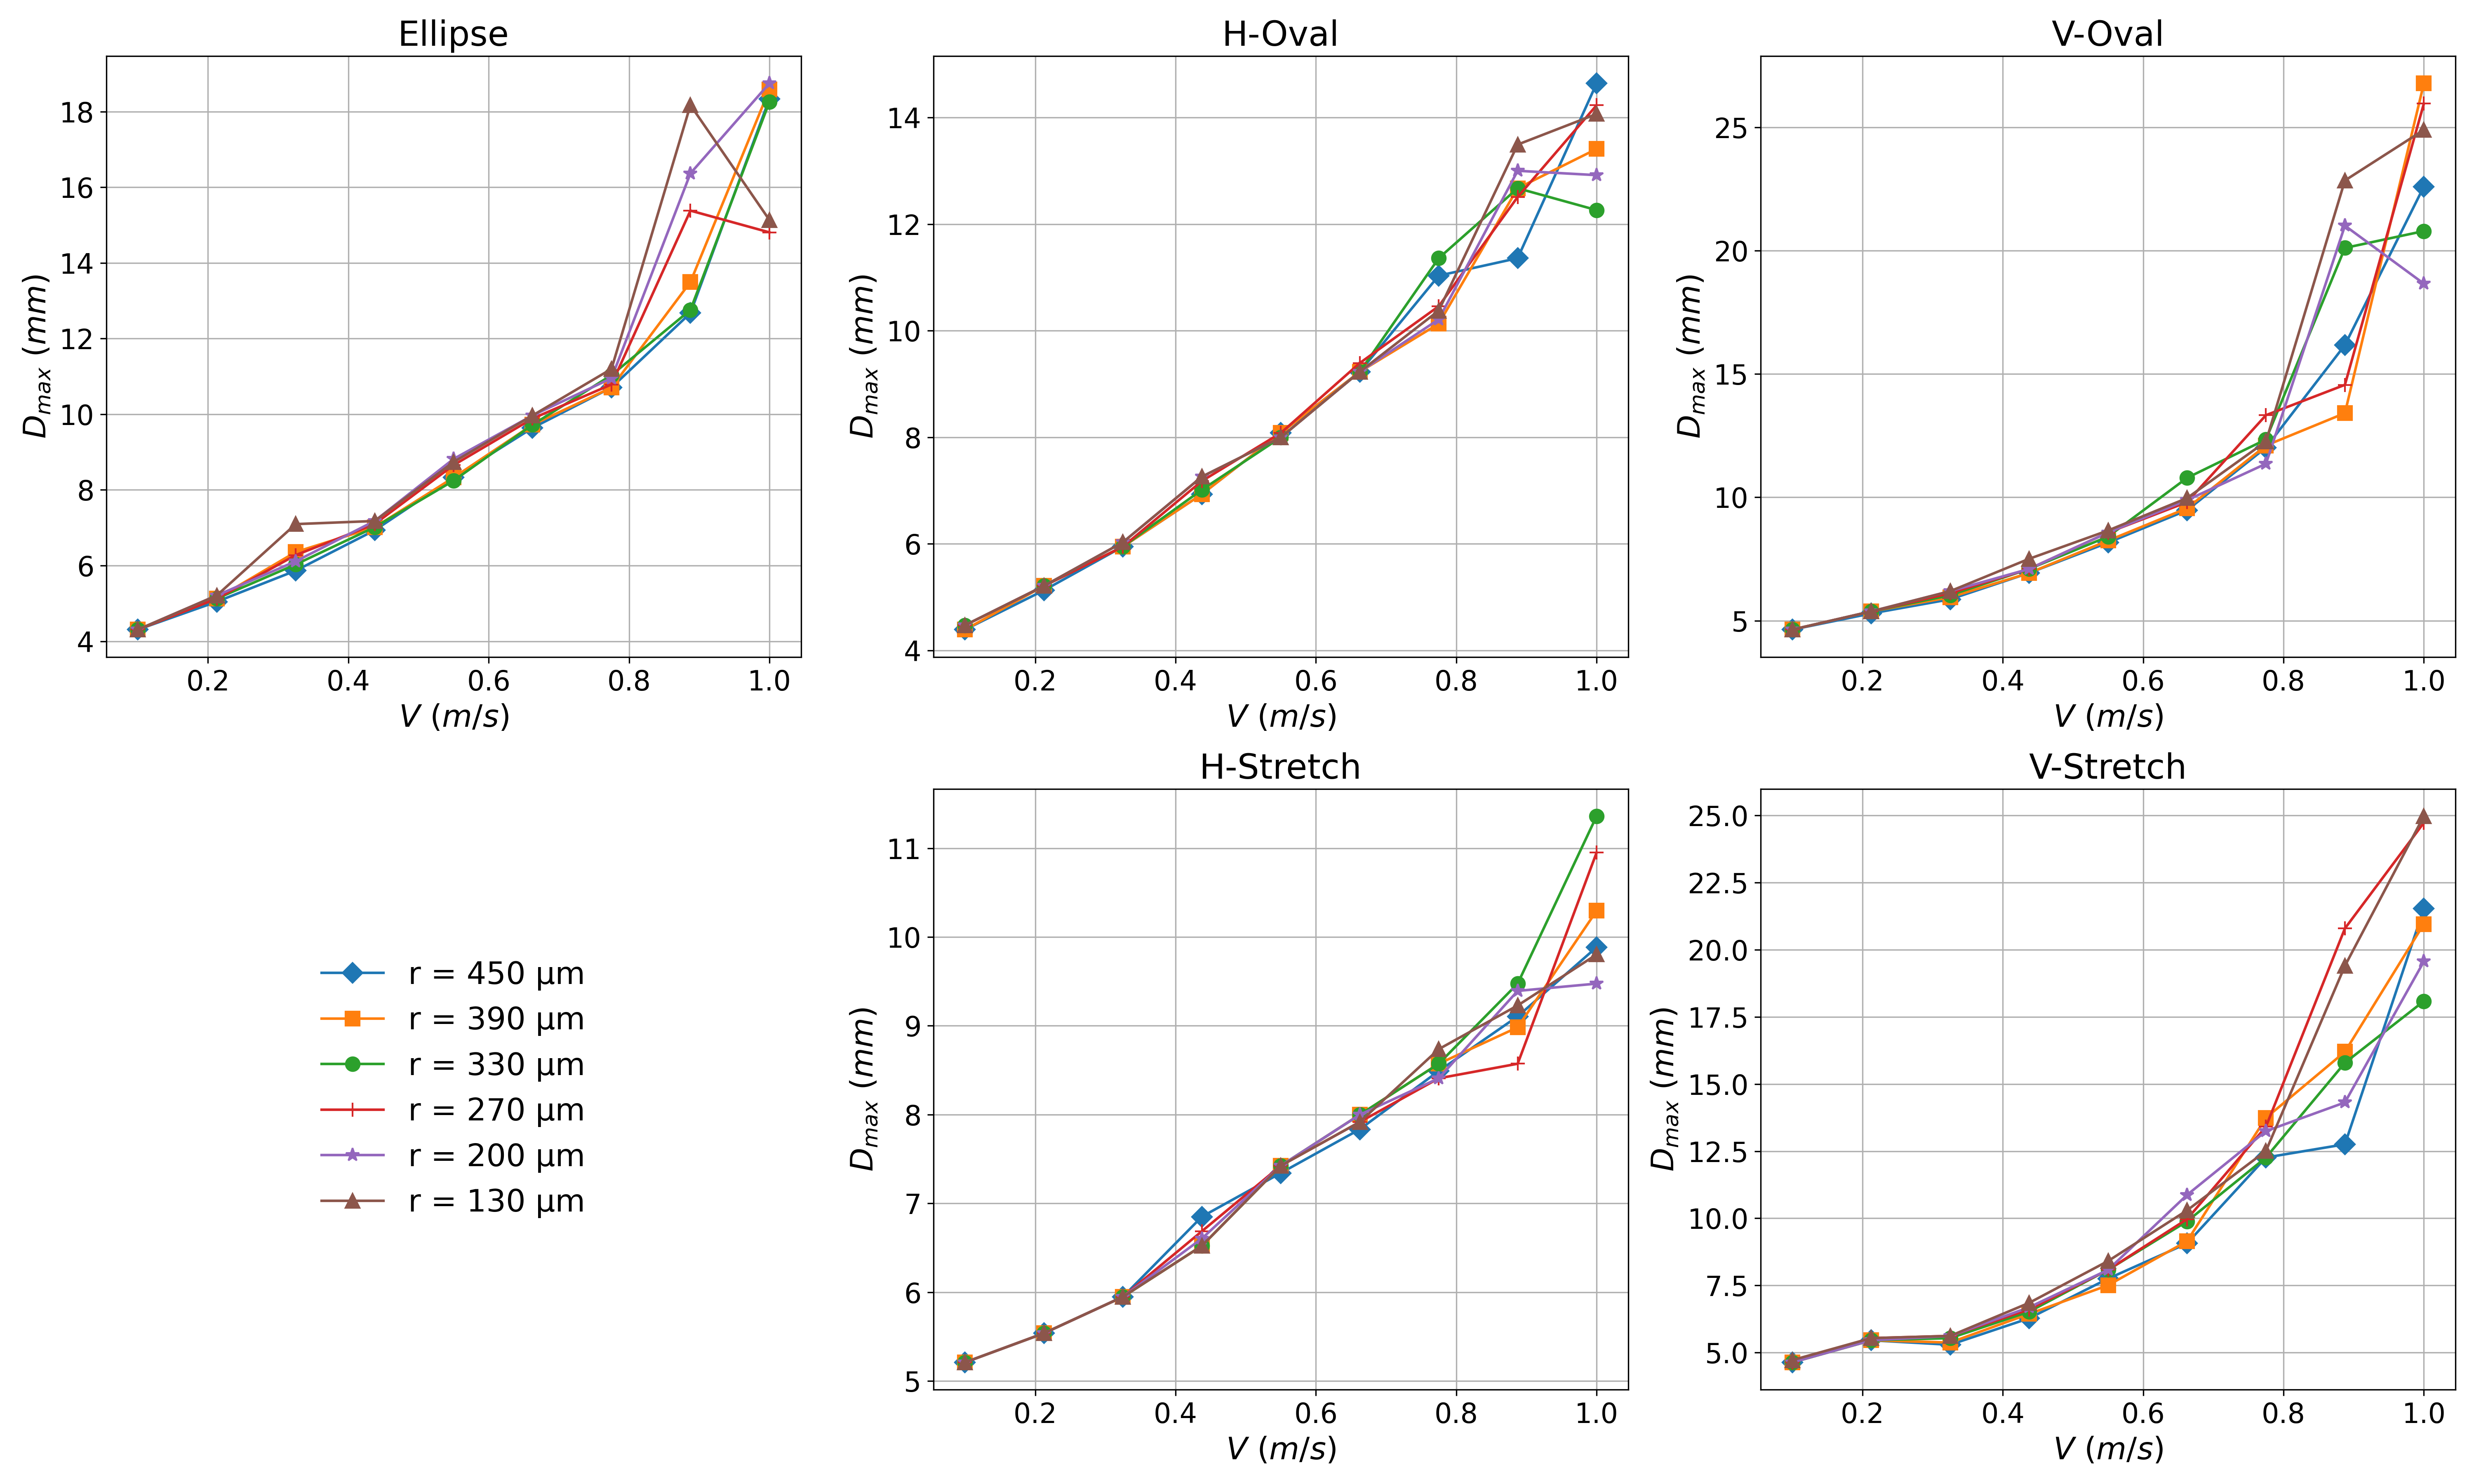
\includegraphics[width=\linewidth]{figures/shape/visc0.0005/grafico4_diametro_maximo_vs_V_dados_0.0005}
        \caption{Maximum horizontal diameters at $\mu = 0.5$ \si{\milli\pascal\second}.}
        \label{fig:diametro_maximo_0.0005}
    \end{subfigure}
    \hfill
    \begin{subfigure}[b]{0.32\textwidth}
        \centering
        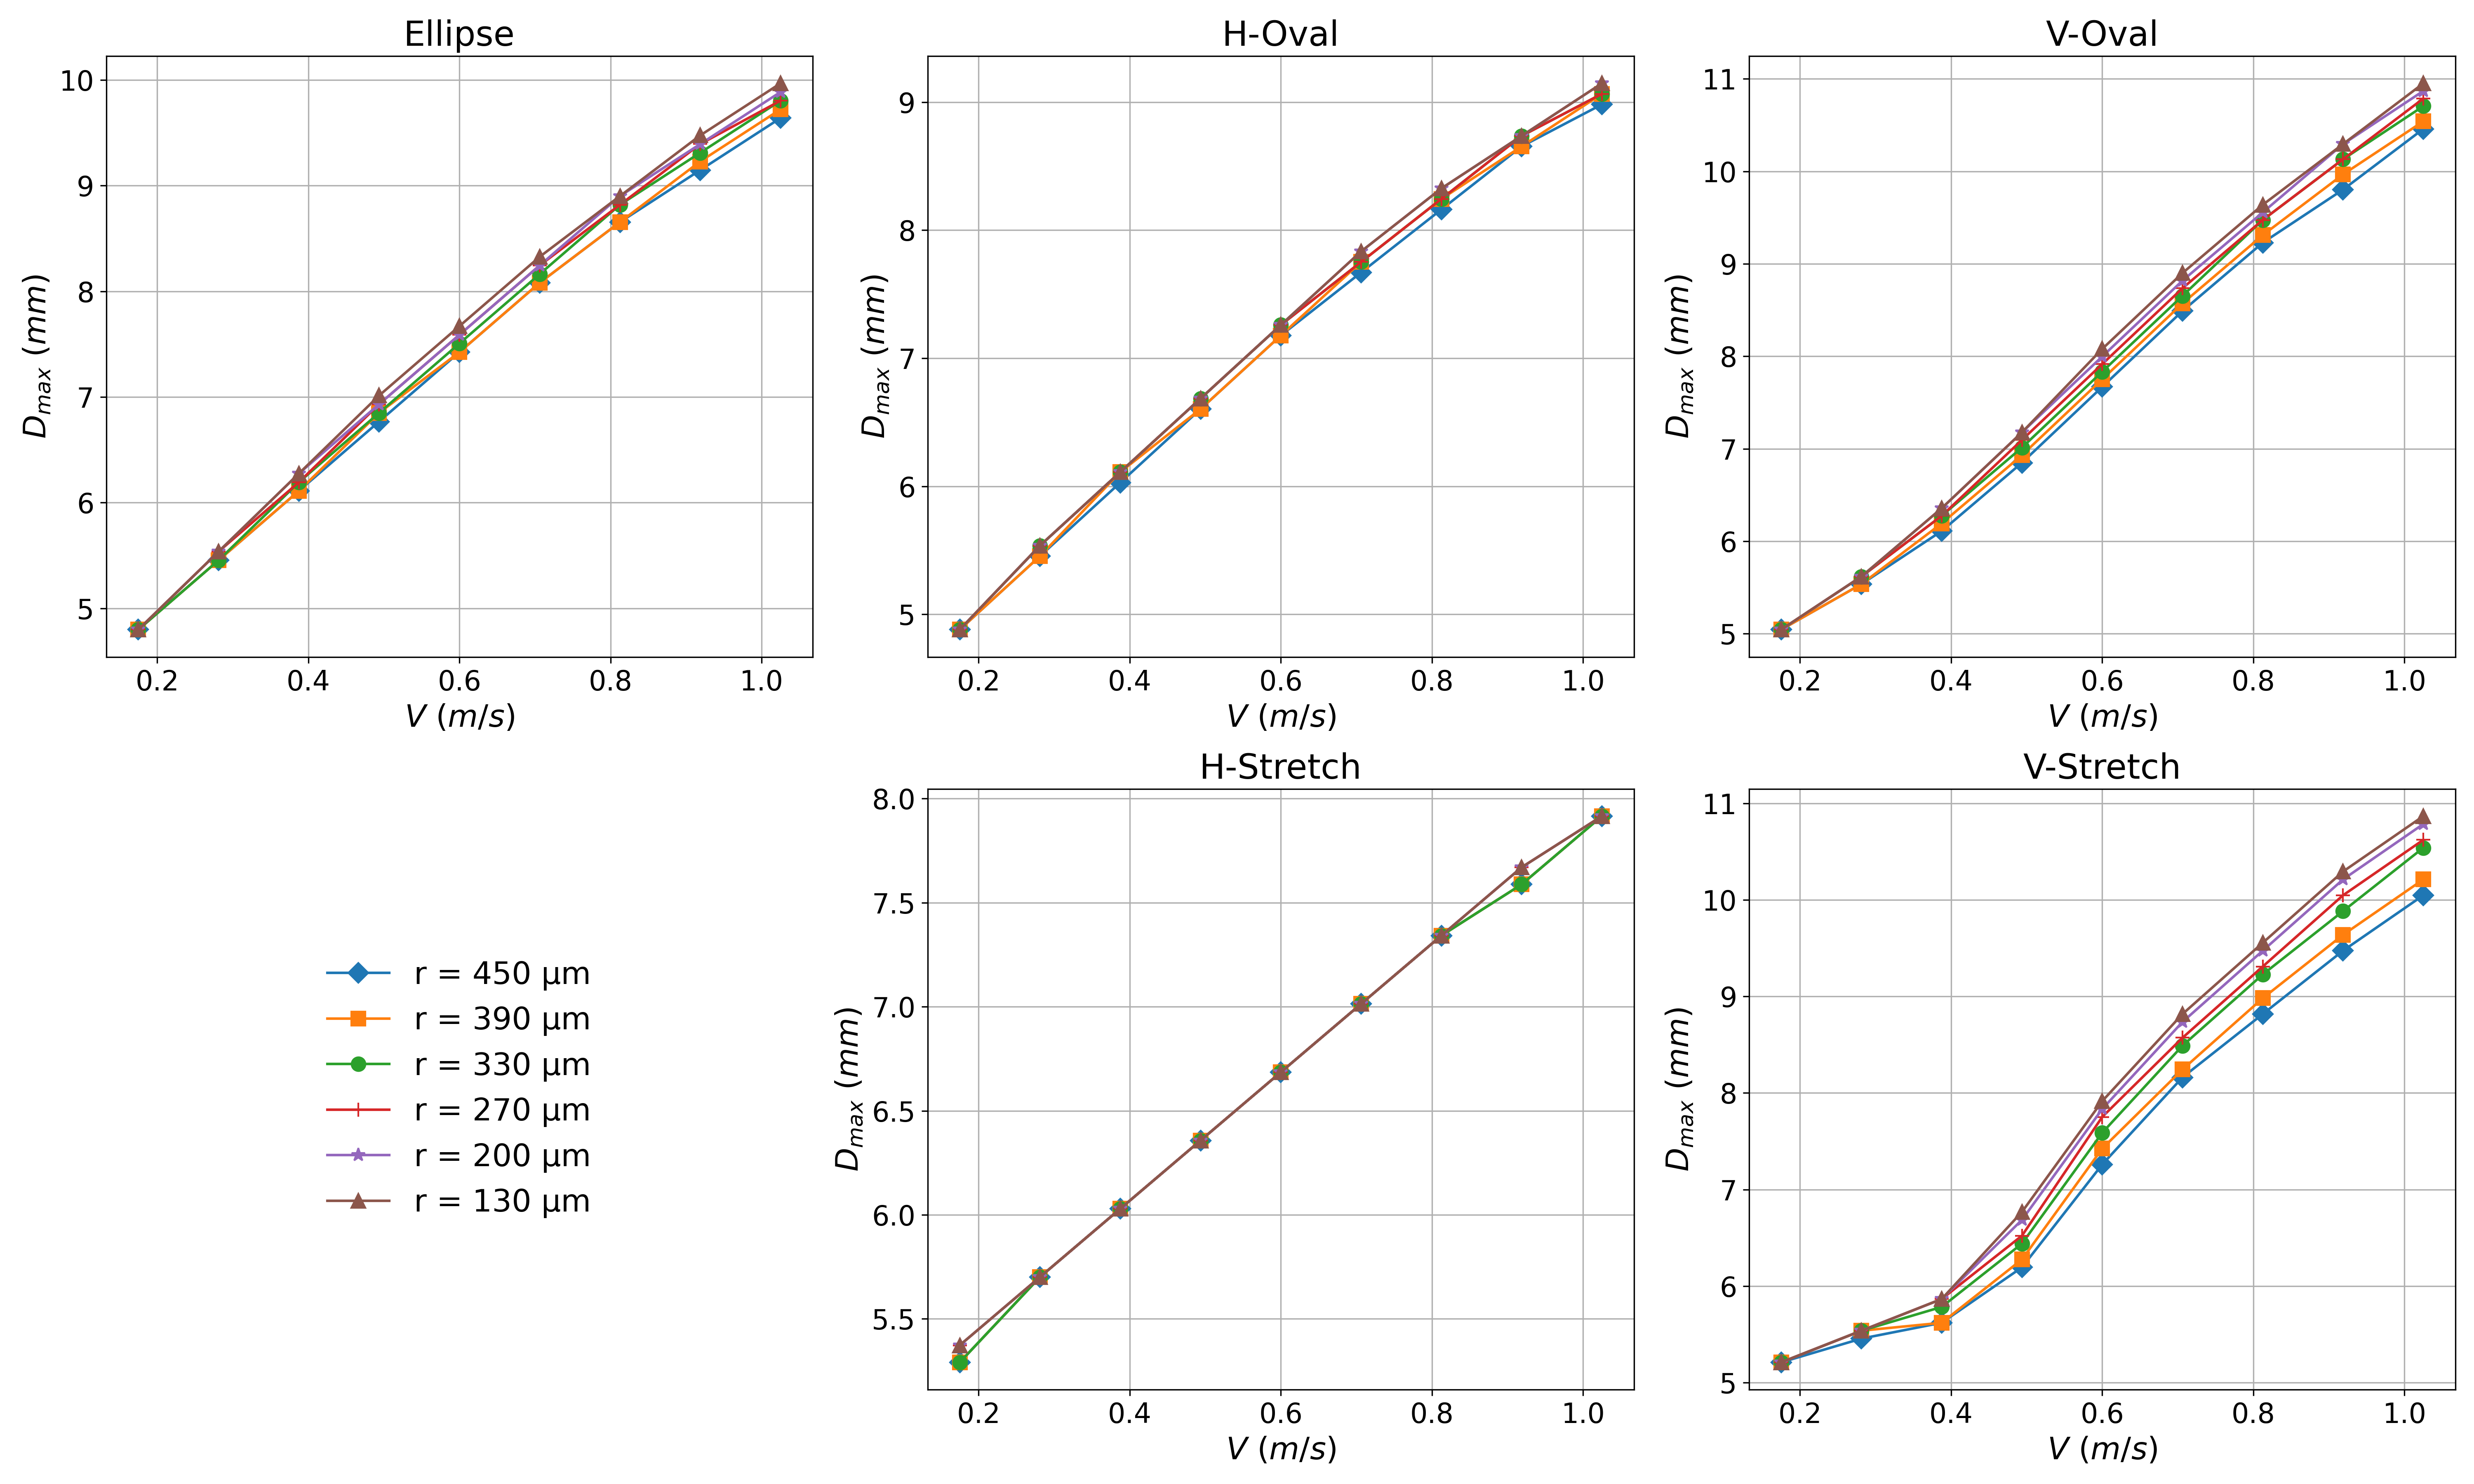
\includegraphics[width=\linewidth]{figures/shape/visc0.005/grafico4_diametro_maximo_vs_V_dados_0.005}
        \caption{Maximum horizontal diameters at $\mu = 5$ \si{\milli\pascal\second}.}
        \label{fig:diametro_maximo_0.005}
    \end{subfigure}
    \hfill
    \begin{subfigure}[b]{0.32\textwidth}
        \centering
        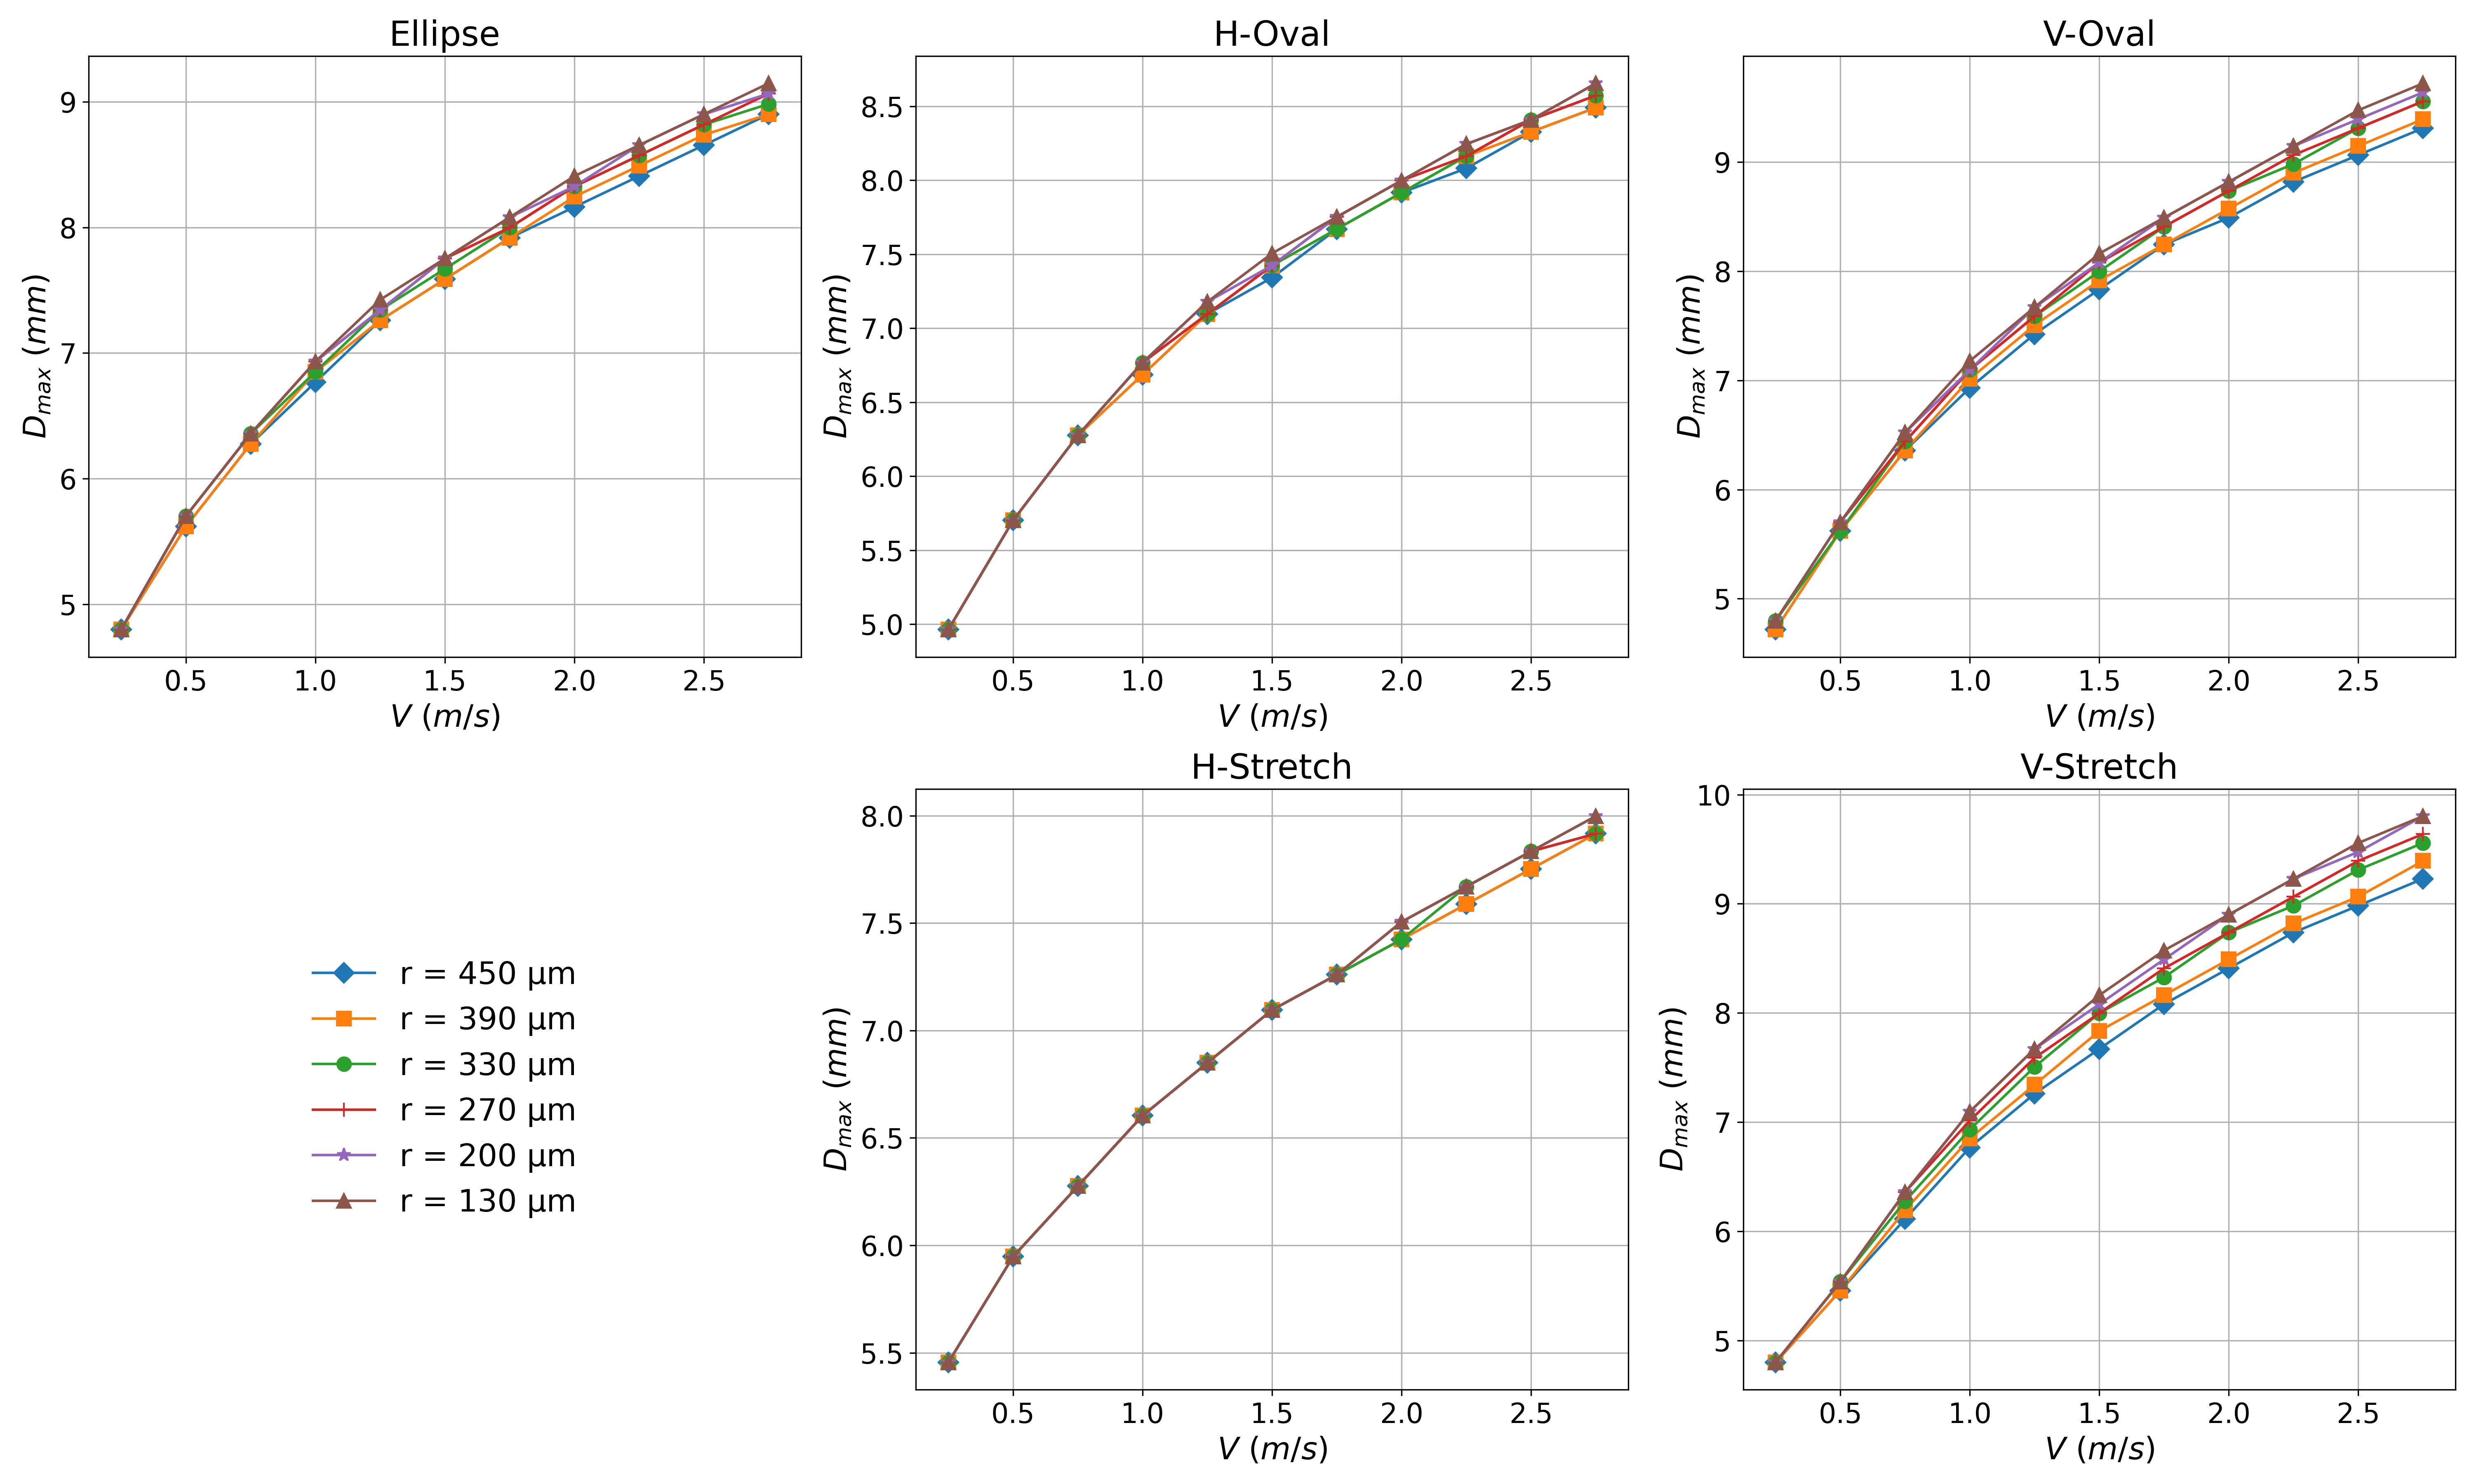
\includegraphics[width=\linewidth]{figures/shape/visc0.05/grafico4_diametro_maximo_vs_V_dados_0.05}
        \caption{Maximum horizontal diameters at $\mu = 50$ \si{\milli\pascal\second}.}
        \label{fig:diametro_maximo_0.05}
    \end{subfigure}
    \caption{Maximum droplet diameter ($D_{\max}$) versus the impact velocity for the five initial droplet shapes and six hole radii at selected impact velocities for viscosities of (a) 0.5, (b) 5 and (c) 50 \si{\milli\pascal\second}.}
    \label{fig:diametro_maximo}
\end{figure}

\subsection{Above the threshold velocity}

Finally, an analysis is conducted exclusively for cases in which breakup occurs, corresponding to impact velocities above the breakup threshold. The analysis focuses on the breakup time ($t^*$) and the maximum vertical elongation of the droplet during penetration ($L$), prior to breakup.

\begin{figure}[!h]
    \centering
    \begin{subfigure}[b]{0.32\textwidth}
        \centering
        \includegraphics[width=\linewidth]{figures/shape/visc0.0005/}
        \caption{μ = 0.5 \si{\milli\pascal\second}.}
        \label{fig:}
    \end{subfigure}
    \hfill
    \begin{subfigure}[b]{0.32\textwidth}
        \centering
        \includegraphics[width=\linewidth]{figures/shape/visc0.005/}
        \caption{μ = 5 \si{\milli\pascal\second}.}
        \label{fig:}
    \end{subfigure}
    \hfill
    \begin{subfigure}[b]{0.32\textwidth}
        \centering
        \includegraphics[width=\linewidth]{figures/shape/visc0.05/}
        \caption{μ = 50 \si{\milli\pascal\second}.}
        \label{fig:}
    \end{subfigure}
    \caption{.}
    \label{fig:}
\end{figure}

{\color{purple}
Falta adicionar ainda:
\begin{itemize}
    \item Resultados do tempo de quebra $t^{*} \times V$ ({\it time of pinch off})

    \item Comprimento máximo $L_{max} \times V t_{R}$.

\end{itemize}
}

% \begin{figure}[!h]
%     \centering
%     \begin{subfigure}[b]{0.32\textwidth}
%         \centering
%         \includegraphics[width=\linewidth]{figures/shape/visc0.0005/}
%         \caption{μ = 0.5 \si{\milli\pascal\second}.}
%         \label{fig:}
%     \end{subfigure}
%     \hfill
%     \begin{subfigure}[b]{0.32\textwidth}
%         \centering
%         \includegraphics[width=\linewidth]{figures/shape/visc0.005/}
%         \caption{μ = 5 \si{\milli\pascal\second}.}
%         \label{fig:}
%     \end{subfigure}
%     \hfill
%     \begin{subfigure}[b]{0.32\textwidth}
%         \centering
%         \includegraphics[width=\linewidth]{figures/shape/visc0.05/}
%         \caption{μ = 50 \si{\milli\pascal\second}.}
%         \label{fig:}
%     \end{subfigure}
%     \caption{.}
%     \label{fig:}
% \end{figure}



%##########%
%Conclusion
%##########%
\section{Conclusion}\label{conclusion}

%###############%
%Acknowledgments
%###############%
\subsection*{Acknowledgments}
I.L. Palhares Junior would like to acknowledge support from  CEPID-CeMEAI (FAPESP Grant No. 2013/07375-0) and FAPESP-SPRINT Grant No. 2024/01651-0 and FAPESP-ANR Grant No. 2024/04769-1.
%I.L. Palhares Junior would like to acknowledge support from  CEPID-CeMEAI (FAPESP Grant no. 2013/07375-0).

%############%
%Bibliography
%############%
\bibliographystyle{abbrv}
\bibliography{bibliography}

%\printbibliography

\end{document}